% The \DocumentMetadata command is used to activate LaTeX3 features
\DocumentMetadata{}
\documentclass[a4paper, 11pt]{report}

\usepackage[draft]{latexcourse}
\usepackage{tocbibind}
\makeindex

\title{A second course in \LaTeX}
\author{Petri Laarne\\University of Helsinki}
\date{\today}


\begin{document}

\maketitle

\tableofcontents

% Each chapter is in its own file.
% This is commonly discouraged in e.g. article manuscripts,
% and might be an overkill even for a (short-ish) dissertation,
% but I personally find it easier in my workflow.
\chapter*{Introduction}
\addcontentsline{toc}{chapter}{Introduction}

\todo{Write up this}

\todo{License and source code availability}

% !TeX root = 2nd-course-in-latex.tex
% (The appearance of \documentclass in the examples confuses LaTeX Workshop for VS Code)

\chapter{Programming}

What really is \LaTeX?

It all starts with \TeX, the typesetting system designed by Donald Knuth in late 70s and 80s.
\TeX{} is a powerful system for laying out text,
but it puts a lot of responsibility on the writer.
Essentially, you are responsible for both the content and its presentation.

\LaTeX{} (originally by Leslie Lamport, now maintained by several people)
extends this core by introducing commands like \cmd{section}:
this command not only lays out the section title in a bigger font,
but also adds some vertical whitespace around it, updates the current section number,
adds an entry to the table of contents, and so on.
This \emph{separates the content from how it is presented}.

We will try to emphasize this philosophy on this course.
By using standard constructs, packages, and our own custom commands,
we can make the \verb|.tex| source code \emph{semantically} meaningful:
something that you could read aloud.
The system then makes sure that the output looks great on paper
-- isn't that why we ever wanted computers to exist!


\begin{warning}
Even when using \LaTeX{}, the old \TeX{} is still there.
It is possible to use plain-\TeX{} commands in your documents,
but \emph{this is highly discouraged}.
These commands sidestep all the enhancements brought by \LaTeX,
and might cause hard-to-diagnose problems.
You might need them when writing more complicated packages,
but then you are already solidly in the ``you are free to shoot your own foot'' territory.
Some such commands are noted in these Warning boxes.

Unfortunately, many heritage templates and Stack Exchange answers still mix
\TeX{}, \LaTeX, and pre-1994 \LaTeX.
Examples of the latter include the obsolete \obscmd{bf} and \obscmd{it} commands
(e.g.\ writing \verb|{\bf bold}| instead of \verb|\textbf{bold}|).
\end{warning}


\begin{latexthree}
The ``standard'' \LaTeX{} version is $2\varepsilon$, released in 1994.
\LaTeX3 is a long-running project (started already before $2\varepsilon$, and reactivated around 2018)
on rewriting the internals of \LaTeX{} to be more extensible.

\LaTeX3 introduces new commands for defining commands and environments.
We will only discuss the version $2\varepsilon$ methods (which are still valid) here,
but if you find yourself writing a package, you should consider learning about the new methods.%
\footnotemark

We will talk about some new features and accessibility improvements brought by \LaTeX3 below,
starting already in \Cref{sec:document structure}.
\end{latexthree}
\footnotetext{\url{www.latex-project.org/help/documentation/usrguide.pdf}}



%
%
%
\section{How \LaTeX{} processes files}

The design of the \TeX{} compiler is limited by the era it was conceived in.
Computer memory was a scarce resource in the 1980s,
so the compiler remembers as little as possible.

In particular, \TeX{} reads its source files from top to bottom.
It never backtracks,
which makes it impossible to reference things that have not yet been defined.

How is it then possible to create cross-references to upcoming sections?
Whenever a \cmd{label} command is encountered,
its name and position is recorded to an \verb|.aux| file.\index{aux file@.aux file}
\LaTeX{} reads in this file before it starts processing the \verb|.tex| file.

Consequently:
\begin{enumerate}
\item On the first compilation, an \verb|.aux| file is generated.
\item On subsequent compilations, cross-references are resolved
    using the \verb|.aux| file from the preceding compilation.
\item This means that all page number references point to \emph{the state of the previous compilation}.
\item Since the resolution might change page numbering,
    it might be necessary to iterate.
    \LaTeX{} gives the
    ``\texttt{Label(s) may have changed. Rerun to get cross-references right.}''
    warning if this is the case.
\item For well-behaved documents, at most three compilations should give convergence.
\end{enumerate}

\begin{warning}
Sometimes, a typo'ed command might end up messing the \verb|.aux| file.
In this case, fixing the error and recompiling will not be enough,
since the \verb|.aux| file feeds back incorrect data.

Usually, the \verb|.aux| file from the recompilation is no longer erroneous,
so a second recompilation is enough.

Rarely, the state might be so messed that the \verb|.aux| file gets re-corrupted
before the compilation halts.
This manifests itself as weird compilation errors even
when you have reverted your code back to a known good state.
If this happens, delete the auxiliary files and recompile from scratch.
Some \LaTeX{} editors have even a handy button for this.
\end{warning}

Since this is the only mechanism for creating forward references,
the \verb|.aux| file is not the only one of its kind.
Some other temporary files that you can expect to see in your compilation folder:
\begin{description}
\newcommand{\filetype}[1]{\item[\texttt{.#1}]\index{#1 file@.#1 file}}
\filetype{bbl} The bibliography generated by the bibliography compiler.
    See below and \Cref{sec:bibliography}.
    Some publishers, in particular arXiv,
    require you to submit this file together with your source code.
\filetype{idx} Index created by the \prg{makeindex} program (\Cref{sec:index}).
\filetype{lof} List of figures.
\filetype{log} This is the raw compiler log.
    \LaTeX{} editors parse this into a more readable form,
    but long, multi-line error messages can be easier to read from the raw log.
\filetype{lot} List of tables.
\filetype{synctex.gz} This is used by some editors to synchronize
    the scrolling of PDF and source code.
\filetype{thm} Theorems (\pkg{ntheorem} package).
\filetype{toc} Table of contents.
\end{description}
%
This list is not exhaustive;
several packages produce their own auxiliary files.
They generally share the file name of the main \verb|.tex| file.

\begin{technote}
These notes also use this mechanism.
Code examples are written inside the \verb|.tex| source files.
Some special commands write the example to a temporary file,
which is then read twice:
once to print out the code, and then again to evaluate the results.
\end{technote}

These auxiliary files can also be read and written by other programs.
The prime example is the \prg{bibtex} program.\label{bibtex process}
Processing a database of bibliographic entries is too complicated to do
inside the \TeX{} programming environment.
Therefore, a separate program is used.%
\footnote{The newer \prg{biber} compiler used by \pkg{biblatex} package works
in a similar way to that described here.}
It works like this:
\begin{enumerate}
\item You write bibliographic data in a \verb|.bib| file.\index{bib file@.bib file}
    See \Cref{sec:bibliography} for the syntax.
\item You write citation commands in the \verb|.tex| source code.
\item When the \LaTeX{} compiler encounters citations,
    it writes some special commands in the \verb|.aux| file.
\item When the \prg{bibtex} program is invoked, it reads the \verb|.aux| file.
    It creates a combined list of all citations,
    and outputs the commands to typeset a bibliography into the \verb|.bbl| file.
\item When \LaTeX{} is run again,
    it reads the \verb|.bbl| file and prints the bibliography.
\end{enumerate}
%
The \LaTeX{} compiler and \prg{bibtex} are decoupled in the sense that
you only need to run \prg{bibtex} when you need to update the bibliography.

In fact, arXiv does not run any bibliographic compilers at all.
They require you to submit the \verb|.bbl| file created by your preferred compiler.
(This probably has to do with two facts:
1. There is more than one bibliography compiler in wide use.
2. The bibliographic databases can contain a lot of data,
also including uncited works.)



%
%
\subsection{Splitting your source into multiple files}

The \cmd{input} and \cmd{include} commands can be used to include additional \verb|.tex| files.
This makes it possible to e.g.\ write each chapter of a long document in a separate file.

\begin{practices}
While it would sound reasonable to split even articles into section-specific files,
there are two reasons not to do so:
\begin{itemize}
\item If you are sharing files with collaborators,
    the complexity of keeping files in sync grows faster than linear in the number of files.
\item Many journals prefer to have the submission in one \verb|.tex| file
    for similar logistical reasons.
\end{itemize}
%
As we see below, there can also be some complexity in setting up the editor.

Therefore my recommendation is:
only split the document if you are preparing a book.
This advice might be extended to theses, and lecture notes
edited by a limited amount of people simultaneously.
These very notes are split into one file per chapter.\footnotemark

When I started preparing this course,
this was the piece of advice I got the most from other \TeX{}nicians.
Consider yourself warned.
\end{practices}
\footnotetext{And suffer from some associated problems.
The ``main file detection'' heuristics of my editor do get confused by this chapter
where several \texttt{\textbackslash documentclass} commands appear.}

There is a minor difference in the two commands.
When \cmd{input} is called with the name of a \verb|.tex| file,
the compiler acts as if the contents of the file were placed in that position.
You could replace the input operation by copy-pasting the file contents.%
\footnote{Some environments do not allow \texttt{\textbackslash input} inside them.}

On the other hand, \cmd{include} finishes the current page
before processing file contents.
This involves placing any queued floats (see \Cref{sec:floats}).
That makes it mostly suitable for including separate chapters.
Every included file gets its own \verb|.aux| file.

The \cmd{includeonly} command temporarily restricts the compilation to a subset of the included files.
This can be a neat way to reduce compilation times on a long document.
Since each file has its own \verb|.aux| file,
cross-references to uncompiled chapters might work (but be outdated!).

\begin{ExampleCode}
% Preamble
\includeonly{intro,discussion}

\chapter*{Introduction}
\addcontentsline{toc}{chapter}{Introduction}

\todo{Write up this}

\todo{License and source code availability}
 % Input intro.tex
\include{methods} % Input methods.tex
\include{results} % Input results.tex
\include{discussion} % Input discussion.tex
\end{ExampleCode}

\begin{gotcha}
\cmd{include} only produces a warning if it cannot find the specified file.
Also, some packages work unreliably with \cmd{include}.

Do not use \cmd{includeonly} when preparing the final copy of your document,
since some of the \verb|.aux| files could be outdated.
\end{gotcha}

\begin{practices}
If you separate chapter contents into their own files,
I highly recommend keeping the ``main file'' very short
-- consisting only of the preamble and \cmd{include} commands.
\end{practices}

In either case,
the included \verb|.tex| file must not contain a preamble --
there already was one in the main file.
Conversely, this means that the separated files cannot be compiled on their own.

There might be some editor-specific support for setting the main file of your project.
This allows you to hit \emph{Compile} while editing a chapter file,
and the main file gets compiled instead.

\begin{overleaf}
You can set the main file in the settings menu at top left of the editor.
\end{overleaf}




%
%
%
\section{Commands and environments}

\begin{practices}
When should you define your own commands?
Generally, the less customization you have,
the easier your manuscript is for the journal publication process and your coauthors.
At the same time, good commands make the code semantically meaningful.

I personally find \verb&\norm{...}& easier to read than \verb&\left\|...\right\|&,
and \verb|\Prob| certainly better than \verb|\mathbb P|,
but others could find those an overkill.
This is a hard balance to strike.

There is just one strict rule:
never repurpose the name of an existing base \LaTeX{} command.
It will cause endless trouble when the journal style or some package tries to use the original command.
\end{practices}


\subsection{Defining commands}
\index{macros}
\TeX{} is a macro language.
This means that there are special source code tokens (\emph{macros}),
that are \emph{expanded} into sequences of more tokens
(including more macros, which are expanded recursively).
The core system includes only a few commands for manipulating internal state and putting out text,
and the rest is achieved via macro expansion.

That was a mouthful, so let us see an example.
In \LaTeX{} macros are defined with the \cmd{newcommand} command.

\begin{VerbatimOut}{\jobname.tmp}
\newcommand{\hello}{Hello world!}

\hello
\end{VerbatimOut}
\ShowExample

Here \cmd{newcommand} takes two arguments:
the first is the name of the macro to define, and the second is what the macro expands to.
In \TeX{} things are grouped with the \verb|{}| braces.
(The first set of braces is technically unnecessary, but it looks cleaner in my opinion.)

Let us see another example where the command is used repeatedly,
and also expanded inside other commands:
\indexcmd{MakeUppercase}
\begin{VerbatimOut}{\jobname.tmp}
\newcommand{\hello}{Hello world}

--\hello, they whispered.\\
--I said, \MakeUppercase{\hello}!
\end{VerbatimOut}
\ShowExample

Since the macros are expanded recursively until there is nothing more to expand,
you can write things that are semantically very unclear,
but comprehensible to a computer:
\begin{VerbatimOut}{\jobname.tmp}
\newcommand{\hi}{^\infty}
\newcommand{\underscore}{_}
\newcommand{\lo}{\underscore{i=1}}

\[ \sum\lo\hi \]
\end{VerbatimOut}
\ShowExample
%
The expansion goes something like this:
\begin{enumerate}
    \item \verb|\sum\lo\hi|
    \item \verb|\sum\underscore{i=1}\hi|
    \item \verb|\sum_{i=1}\hi|
    \item \verb|\sum_{i=1}^\infty|
\end{enumerate}
So the end result is the same as if one had written the sum sensibly from the beginning.



\begin{warning}
In plain \TeX{} macros are defined with \obscmd{def} and \obscmd{let}.
If you see code using either,
you have entered the ``shoot your own foot'' territory.\footnotemark
\end{warning}
\footnotetext{Since you asked, the difference between the two is whether the contents of the macro
are expanded at usage or definition time.
Neither protects you against overwriting existing macros.}
\quiettodo{Keep these on the same page!}


The \TeX{} compiler works in two basic modes: text mode and math mode.
Some commands (for example, \verb|\sqrt|) are only usable in math mode.

How to define a command that works \emph{both} in text and math mode?
You can use the \cmd{ensuremath} command: in text mode it wraps its contents inside \verb|$|,
and in math mode it does nothing:
%
\begin{VerbatimOut}{\jobname.tmp}
\newcommand{\magic}{\ensuremath{\sqrt 2}}

The number \magic{} satisfies
\[
\magic^2 = 2.
\]
\end{VerbatimOut}
\ShowExample




%
\subsection{Arguments to commands}

To pass arguments to macros, we can indicate their number with an optional argument
between the macro name and definition.
These arguments can then be accessed in the macro definition with \verb|#1|, \verb|#2|, and so on.

\begin{VerbatimOut}{\jobname.tmp}
\newcommand{\say}[2]{#1 says ``#2''!}

\say{Petri}{Hi}
\end{VerbatimOut}
\ShowExample

Arguments are often wrapped in the \verb|{}| braces,
but it is not actually necessary -- in a very specific case.
By default, \LaTeX{} interprets a single letter or a number as an argument.
The braces extend the argument to a longer stretch.

This means that all of the following are equivalent:

\begin{VerbatimOut}{\jobname.tmp}
\[
\frac{1}{2}
= \frac 1 2
= \frac12.
\]
\end{VerbatimOut}
\ShowExample

Do note the last one -- \LaTeX{} command names can only consist of letters,
so the number 1 is not interpreted as part of the command name but an argument.
There is no requirement to separate the name and a following number.
(I do find the last example hard to read, though.)
Conversely, whitespace won't separate longer arguments; you really need the braces:

\begin{VerbatimOut}{\jobname.tmp}
\[
\frac 12 34
\neq \frac {12} {34}.
\]
\end{VerbatimOut}
\ShowExample

However, commands are interpreted as single tokens.
This happens regardless of whether the command would expand to several tokens.

\begin{VerbatimOut}{\jobname.tmp}
\newcommand{\magic}{314 159}
\[ \frac \magic \pi \]
\end{VerbatimOut}
\ShowExample

\begin{gotcha}
Some built-in macros swallow the whitespace that follows them.
If a word space is actually needed, you can feed the command an empty group \verb|{}|:
\begin{VerbatimOut}{\jobname.tmp}
\LaTeX programming\\
\LaTeX{} programming
\end{VerbatimOut}
\ShowExample
\end{gotcha}


%
\subsection{Groups and scopes}

\index{group}\index{scope}
\label{ex:font scope}
More precisely, the braces delimit a \emph{group}.
A group is handled as a single argument to a command.
Additionally, they serve as a \emph{scope} for commands that change
how all the following text is output.
For example, the font-sizing commands like \cmd{tiny} and \cmd{Large}
affect the size of all text that follows them.
However, this effect only lasts until the group is closed with a \verb|}|.

\begin{VerbatimOut}{\jobname.tmp}
{\tiny I am small}
and I am normal
and {\Large I am large}
\end{VerbatimOut}
\ShowExample

If you forget about this and just write \cmd{tiny} without any scoping,
you will have tiny text until the end of document (or the next font size command).

\begin{VerbatimOut}{\jobname.tmp}
\tiny I am small and
{\Large I am large}
and I am tiny again
\end{VerbatimOut}
\ShowExample

There is one place where the braces do not delimit a group:
in the definition of commands.
In the following example, \verb|\mouse{Squeak}| is expanded into
\verb|\tiny Squeak| and not into \verb|{\tiny Squeak}|.
Therefore the effect persists onto the following line.
%
\begin{VerbatimOut}{\jobname.tmp}
\newcommand{\mouse}[1]{Mouse: \tiny#1.}

\mouse{Squeak}\\
I: Oops.
\end{VerbatimOut}
\ShowExample
%
The scope can be introduced here by adding \verb|{}| into the command definition:
%
\begin{VerbatimOut}{\jobname.tmp}
\newcommand{\mouse}[1]{{Mouse: \tiny#1.}}

\mouse{Squeak}\\
I: Alright.
\end{VerbatimOut}
\ShowExample

Scopes also affect things like \cmd[scope]{newcommand}:
the command \verb|\mouse| defined above only exists
within the example block, and is not accessible beyond it.



%
\subsection{Optional arguments}

Some commands also have optional arguments.
Instead of braces, these are passed within brackets \verb|[]|.
A basic example is the \cmd{sqrt} command
that produces not only square roots, but general roots:
\begin{VerbatimOut}{\jobname.tmp}
$\sqrt{7}$,
$\sqrt[3]{7}$.
\end{VerbatimOut}
\ShowExample

Another example is the optional argument to \cmd{cite} command,
which indicates a precise position within the cited work:
\verb|\cite[Page 40]{TLC}| produces \cite[Page 40]{TLC}.
(Here \verb|TLC| is the bibliography key for \emph{The \LaTeX{} Companion};
we will discuss this more in \Cref{sec:bibliography})

\begin{gotcha}
Inside an optional argument, \LaTeX{} interprets the first \verb|]| it sees as the closing bracket.
This means that if you need to use \verb|[]| \emph{inside} an optional argument
(say, as an optional argument to an inner command), you need to wrap things in braces.
Quite often, you might need even \emph{two sets of braces}.
Compare the two citations:
%
\begin{VerbatimOut}{\jobname.tmp}
\cite[{{Page [40] maybe?}}]{TLC}\\
\cite[Page [40] maybe?]{TLC}
\end{VerbatimOut}
\ShowExample
%
The first citation is shown correctly.
In the second, the optional argument is interpreted to be ``\verb|Page [40|''
and the citation name then ``\verb|m|'' (only a single letter since it was not wrapped in braces).
The remaining ``\verb|aybe?]{TLC}|'' is then normal body text.
\end{gotcha}

\begin{gotcha}
\LaTeX{} ignores whitespace between a command and its optional argument.
This might sometimes lead to surprising behaviour.
Here the second list item is interpreted as an optional argument that replaces the bullet symbol:
\indexcmd{item}
%
\begin{VerbatimOut}{\jobname.tmp}
\begin{itemize}
\item Cookies
\item [Maybe cake?]
\item Drinks
\end{itemize}
\end{VerbatimOut}
\ShowExample
\end{gotcha}


The syntax for optional arguments is not always clear:
sometimes they precede the real arguments, sometimes they follow them.
Sometimes they consist of just one thing,
sometimes they can be a list of things
(see the discussion of \cmd{usepackage} later in this chapter).


%
\subsection{Replacing existing commands}

Sometimes it is useful to overwrite an existing command.
One common example is rewriting \cmd{epsilon} to actually mean \cmd{varepsilon},
since many consider the variant $\varepsilon$ prettier than the regular $\epsilon$.

It is not possible to write \verb|\newcommand{\epsilon}{\varepsilon}|,
since \LaTeX{} rightly complains about \verb|\epsilon| being already defined.
You could be accidentally overwriting a command used elsewhere in the document.
You have to make your intentions clear by using \cmd{renewcommand}:

\begin{VerbatimOut}{\jobname.tmp}
Old epsilon: $\epsilon$,\\
\renewcommand{\epsilon}{\varepsilon}
New epsilon: $\epsilon$.
\end{VerbatimOut}
\ShowExample
%
Again, the redefinition of a command lasts only for the current scope.
Once the scope is closed, \verb|\epsilon| again means the old regular symbol.
To redefine a command within the entire document,
you need to call \cmd{renewcommand} in the document preamble.

Here is an example of \cmd{newcommand} and \cmd{renewcommand} with arguments.
The two commands have matching syntax.
Note that the new definition is free to have a different number of arguments.

\begin{VerbatimOut}{\jobname.tmp}
\newcommand{\dual}[2]{(#1 \mid #2)}
Mathematicians: $\dual{a}{b}$.\\
\renewcommand{\dual}[2]
  {\langle#2 \mid #1\rangle}
Physicists: $\dual{a}{b}$.
\end{VerbatimOut}
\ShowExample

The \cmd{DeclareCommandCopy} robustly copies the current definition of a command.%
\footnote{This can also be done with raw \TeX{} primitives, which are to be avoided.}
It is then possible to renew the definition, and still access the previous version.
Let us illustrate this by swapping the meanings of \verb|\epsilon| and \verb|\varepsilon|:
%
\begin{VerbatimOut}{\jobname.tmp}
Epsilon $\epsilon$ and varepsilon $\varepsilon$

\DeclareCommandCopy{\oldepsilon}{\epsilon}
\DeclareCommandCopy
    {\oldvarepsilon}{\varepsilon}
\renewcommand{\epsilon}{\oldvarepsilon}
\renewcommand{\varepsilon}{\oldepsilon}

Epsilon $\epsilon$ and varepsilon $\varepsilon$
\end{VerbatimOut}
\ShowExample

\begin{latexthree}
This command is part of the \LaTeX3 programming interface.
It requires a relatively recent (2020 or later) \LaTeX{} version.
\end{latexthree}


%
\subsection{Defining environments}

\index{environments}
Environments encapsulate larger blocks of text.
They also form implicit groups.

\begin{VerbatimOut}{\jobname.tmp}
\begin{center}
\renewcommand{\epsilon}{\varepsilon}
Centered text and $\epsilon$
\end{center}

\begin{flushright}
Right-aligned text.
Here we have the old $\epsilon$.
\end{flushright}
\end{VerbatimOut}
\ShowExample

To define an environment, we use the \cmd{newenvironment} command.
This command takes three arguments: the name of the environment
and code to expand at the beginning and the end of the environment.

\begin{VerbatimOut}{\jobname.tmp}
\newenvironment{cool}
    {A mathmo enters the lab.\par}
    {\par The mathmo leaves the lab.}

\begin{cool}
A massive explosion occurs.
\end{cool}
\end{VerbatimOut}
\ShowExample
%
(If you're wondering about the \cmd{par} commands,
they are used to ensure that the first and last lines are their own paragraphs.)

There is also \cmd{renewenvironment} that works like \verb|\renewcommand|.

Since environments are groups,
it is possible to change font characteristics for the duration of the environment:

\begin{VerbatimOut}{\jobname.tmp}
\newenvironment{mouse}{\tiny}{}

Ordinary text.
\begin{mouse}
Very small and very squeaky text.
\end{mouse}
Again ordinary text.
\end{VerbatimOut}
\ShowExample
%
Note that here the end code is empty;
the font properties are reset automatically as the group ends.

\begin{gotcha}
If the begin/end code of your environment spans multiple lines,
you need to be careful with line breaks.
The extra whitespace might cause \LaTeX{} to output an unintended empty space
or even a paragraph break.
To avoid line breaks to be interpreted as line breaks,
you can end each line in the environment definition with \verb|%|
-- the comment character shallows the line break.

This same thing applies to empty lines before and after environment usage
-- the usual paragraph-breaking rules apply.
If you don't want to start a new paragraph after the environment ends,
do not leave an empty line between \verb|\end{...}| and the following text.
(For visual separation in the code, I prefer a line containing just \verb|%|.)
\end{gotcha}




%
%
%
\section{Diagnosing errors}

Macro languages were popular in the 1980s, back when 640 kilobytes was enough memory for anyone.
An unfortunate consequence of \TeX's stability is that the compiler still operates under this worldview.
The source code is read exactly once from top to bottom,
and if the code is not correct, error messages can be extremely cryptic.

\begin{overleaf}
Some \LaTeX{} distributions are set up to ignore some errors.
For example, Overleaf is quite good at ignoring missing \verb|$| signs and other small typos.
You should really pay attention to red symbols in the source code margin
and next to the \emph{Recompile} button!
\end{overleaf}

The compiler gives three forms of output: information, warnings and errors.
Graphical \LaTeX{} editors usually only show the latter two.
(Information is printed in the console output.
It includes the current source file and page number that the compiler is processing,
which can help diagnose a stuck compilation.)

\index{warnings}
Warnings are just as the name says: the document can still be compiled,
but you should check whether you have gotten what you intended.
Generally, the warning messages are very descriptive:

\medskip\noindent\emph{Overfull or underfull hbox.}\\*
A line could not be breaked in a nice way.
See \Cref{sec:overfull} for how to solve this.

\medskip\noindent\emph{Citation or label undefined.}\\*
\LaTeX{} could not recognize a label that you tried to reference.
If the label or bibliography entry was newly added, a recompilation might fix this.
Otherwise you have forgotten to define it at all, or just forgotten how to spell it.
See \Cref{sec:crossref,sec:bibliography}.

\medskip\noindent\emph{Label(s) may have changed. Rerun to get cross-references right.}\\*
Indeed, you have added a new label since the last compilation.
Just recompile the file.

\medskip\noindent\emph{Temporary extra page added at the end. Rerun to get it removed.}\\*
This can happen if the document becomes shorter than in the last compilation.
\LaTeX{} tries to place the processing that happens at \verb|\end{document}|
to the final page, but it does not know the final number of pages until it is too late
(hence it looks at the previous compilation for a hint).
As the message says, there is an extra page explaining the issue at the end.
Recompile and it goes away.


\begin{practices}
You should always check for warnings before submitting a document.
It's a bit embarrassing to publish a document with [\textbf{?}] citations, after all.

Overfull and underfull hboxes are usually \emph{not worth fixing}
until the final typesetting phase,
since very small changes to the text or style can drastically change the line breaking.
\end{practices}


\index{errors}
Errors, on the other hand, halt the compiler altogether.
The compiler can try to ignore errors and recover itself,
but at that point \emph{it is guessing} what you tried to mean,
and might get even more confused.
Quite often the internal state is so messed up, \TeX{} can only spew more errors.


\begin{practices}
Recompile often.
It is much easier to locate an error when you have modified only a small region of the code.

Always recompile after you modify a command definition
or do a find-and-replace operation.
These are risky.

If your document takes a long time to compile,
find a way to speed it up
(skip complicated TikZ pictures in draft mode, only include chapters you're working on, etc.).
If recompilation breaks your flow, you won't do it often enough.

For some pointers for conditionally skipping parts of pictures, see page~\pageref{ex:booleans}.
\end{practices}


\medskip\noindent\emph{[100+ error messages]}\\*
Did you just modify the definition of a command?
If so, then you probably introduced a typo there.

If not, this is a strong sign that \TeX{} failed to recover from an error.
Scroll to the \emph{very first} error message and fix it.
The later error messages are misleading,
and will go away once the actual error is fixed.

If the cause of the error is a command used inside a sectioning command or table specification,
you may have hit a robustness issue; see \Cref{sec:robustness}.

\medskip\noindent{\em \verb|\begin{equation}| on input line 7 ended by \verb|\end{equation*}|}\\*
Exactly what is says: there is a mismatched begin/end combination.
If the message says \verb|\end{document}|, then the end command is missing altogether.

\medskip\noindent{\em Missing \verb|$| inserted}\\*
You have tried to use a math-mode command while in text mode.
If you want to define a custom command that works in both modes,
you can wrap mathematical symbols in it within \cmd{ensuremath}.

\medskip\noindent\emph{Bad math environment delimiter}\\*
Conversely, do you have an extra \verb|$| inside a display math environment?

\medskip\noindent{\em Misplaced alignment tab character \verb|&|}\\*
\medskip\noindent{\em Extra alignment tab has been changed to \verb|\cr|}\\*
You have a bit too many \verb|&| characters per line,
or are using an equation environment that does not support them at all.

\medskip\noindent{\em Package amsmath Error: \verb|\begin{split}| won't work here.}\\*
You need to wrap the environment inside \verb|equation| or one of its friends.

\medskip\noindent\emph{Missing character: There is no \emph{\dots} in font nullfont!}\\*
If this happens inside a TikZ picture, you have very likely mistyped a command or option.
Check the code line shown above the error message.

\future{More common error messages}



%
%
%
\section{Document structure}\label{sec:document structure}

Let us then look at the basic structure of a \verb|.tex| file.
Everyone reading these notes is assumed to have seen such a file more than once,
but we will spend some time on some nuances.
Bear with me even if this sounds trivial!

\begin{practices}
I would advocate for starting every project from an empty \verb|.tex| file.
The problem with ``heritage'' templates is that they accumulate a lot
of unnecessary package dependencies and custom commands.
I've seen files where the same package is loaded three times.

By starting from an empty file
and only adding the customizations you need for the particular project,
you help maintain your ``code hygiene''.
\end{practices}

Let us start with the minimal example below.

\begin{ExampleCode}[numbers=left]
\DocumentMetadata{}
\documentclass[a4paper]{article}

\fontencoding{OT1} % Read note below!
\usepackage[hidelinks]{hyperref}

\title{My first document}
\author{Firstname Lastname}
\date{\today}

\begin{document}

\maketitle

% Rest of content here...

\end{document}
\end{ExampleCode}

We discuss the first line in a \LaTeX3 note below.
On the second line, we load a \LaTeX{} document class.
The document class determines the basic layout of your document,
and it is where several basic commands like \cmd{maketitle} are defined.
We will look at some different document classes and arguments in the next subsection.

Lines 1--10 are collectively known as the \emph{preamble}.\index{preamble}
This is the best place to define new commands and do other setup.
Additional packages are also loaded here; see \Cref{sec:loading packages}.

\begin{latexthree}
What's interesting in the above example is the one package that is \emph{not} loaded.
The \pkg{inputenc} package used to be very important to load,
since it told \LaTeX{} about the encoding of non-English characters.
Since 2018 \LaTeX{} has followed the rest of the world
and uses UTF-8 encoding by default.

What does this mean for you?
If you create a new file in any reasonably modern \LaTeX{} editor,
you get the correct encoding and don't need to load \pkg{inputenc}.

However, if you modify a sufficiently aged file that contains non-English characters,
you might stumble upon legacy encodings like \texttt{latin1} or \texttt{cp1252}.
In such files, the \pkg{inputenc} package must be loaded with the proper optional argument.
\end{latexthree}

The \verb|\fontencoding| command tells \LaTeX{} that Unicode characters will appear
not only in the source code, but also the final output
-- thus the font must be interpreted in a compatible way.
However, this command should only be used with the traditional pdfTeX compiler;
if you use the newer LuaLaTeX or XeLaTeX compilers,
this command might cause subtly worse output.
See page~\pageref{rem:font encoding} for more explanation.


Trying to output any text before the \verb|\begin{document}| line is an error.
\indexenv{document}%
When the compiler reaches that line,
a lot of stuff happens behind the scenes to prepare \LaTeX{} for actually outputting pages.

Similarly, the \verb|\end{document}| line is necessary.
At that point, a lot of code is executed to make sure that everything is output properly.
Any text written below that line is ignored.
(I do not recommend writing anything there!)

\begin{latexthree}
An important part of the \LaTeX3 project is revising the PDF output
to include accessibility information:
for example, tagging section headings as headings and not just bold text in big font.
Since this might cause issues with some packages, the new behaviour is opt-in.

If you write \indexcmd{DocumentMetadata}\verb|\DocumentMetadata{}|
before the \verb|\documentclass| declaration, you opt in to these new features.
This command also enables new functionality in e.g.\ the \pkg{hyperref} package.
\end{latexthree}


%
\subsection{Document classes}\label{sec:document classes}

\begin{practices}
Journals commonly define their own document classes, based on one of the standard classes.
The discussion below only applies to the documents where you are in charge of the style.
Always look at the journal instructions for preparing the published version of your article.
\end{practices}

\index{document classes}
There are three document classes of interest included in base \LaTeX{}:

\begin{description}
\item[article] As the name suggests, this should be used for articles, short notes, and such.
    The \cmd{maketitle} command does not create a separate title page,
    and the highest-level sectioning command is \cmd{section}.
    There is no page break between sections.
\item[report] This class is suitable for e.g.\ a thesis, lecture notes, or a longer article.
    The present notes use this class.
    There is a separate title page,
    and the highest-level sectioning command is \cmd{chapter}.
    Each chapter begins on a new page.
\item[book] This is the heaviest of all the classes.
    You get a lot of empty pages, just like in a real printed book.
    If you find yourself using this class,
    you have agreed to something monumental.
\end{description}
%
There is also a \textbf{letter} document class,
which understandably sees little use nowadays.
But it is still there if you need it!

Options passed to document classes are interesting in that
\emph{they are also passed to all packages}.
If you pass \verb|a4paper| to the document class,
then you don't need to pass it again to the \pkg{geometry} package.

Some options are supported by all the basic document classes:

\begin{description}
\item[a4paper] This is self-explanatory.
    By default, \LaTeX{} assumes the American letter paper size.
\item[10pt, 11pt, 12pt] Sets the body font size.
    Fonts for section headers, footnotes, etc.\ are scaled accordingly.
    The default is 10~points.
\item[oneside, twoside] Whether the margins are equal
    or alternating between odd and even pages.
    For example this document (which is aimed for consuption on a screen)
    uses \verb|oneside|, but a printed report should specify \verb|twoside|.
\item[openright, openany]
    Whether chapters always begin on a right-hand side page (default for book)
    or any page (default for report).
    You should consider \verb|openright| for a printed thesis
    and \verb|openany| for electronic version.
    Not applicable to the article class where chapters are not supported at all.
\item[notitlepage, titlepage] Whether the title is set on a separate page.
\item[fleqn] Instead of centering, left-aligns display formulas.
\item[twocolumn] Sets the text in two columns.
\end{description}


A very common alternative document class is \textbf{amsart}.\indexpkg{amsart}
It is developed by the American Mathematical Society,
and some prefer its style to that of \textbf{article}.
It is a drop-in replacement for \textbf{article} and supports the same options.

Other common classes include those from \pkg{koma-script}
(drop-in replacements for all standard classes)
and \pkg{memoir} (intended for longer documents),
which both provide a lot of flexibility.
They both come with extensive documentation for those who wish to venture into that rabbit hole.


%
\subsection{Loading packages}\label{sec:loading packages}

In the previous example, we loaded the \pkg{hyperref} package with:
\begin{ExampleCode}
\usepackage[hidelinks]{hyperref}
\end{ExampleCode}
Options can be passed to packages inside the brackets.
Here we pass the \verb|hidelinks| option that suppresses the coloured boxes around clickable links.
Some packages also take options with a \verb|key=value| notation.

In addition to the options passed explicitly,
all the options passed to the document class are also forwarded to the package.

\begin{practices}
You should always load \pkg{hyperref}.
It not only turns cross-references into clickable links,
but also adds section headers to the PDF table of contents
(usually found in the sidebar of any reader application).
Your readers will appreciate this navigation aid.
\end{practices}

\index{packages!finding}
CTAN, the \emph{Comprehensive \TeX{} Archive Network},
is the repository for \LaTeX{} packages.
It can be browsed at \url{www.ctan.org}.

Generally \LaTeX{} distributions either contain the whole CTAN,
or are able to download packages from there as needed.
You should check out how you can keep your distribution up to date,
as new versions of packages are continually released.

Most importantly, all major packages listed on CTAN have good documentation there.
The documentation typically includes usage examples, a complete reference,
and possible compatibility issues with other packages.
For example, you can find the (very extensive!) documentation of \pkg{hyperref}
at \url{www.ctan.org/pkg/hyperref}.
They are also available at \url{www.texdoc.org}.

\begin{description}
\item[babel] Support for languages other than English.
    See \Cref{sec:babel}.
\item[cleveref] Automatic cross-reference formatting.
    See \Cref{sec:cleveref}.
\item[enumitem] Customization of list structures.
    See \Cref{sec:lists}.
\item[graphicx] Inclusion of image files.
    Replaces the old \obspkg{graphics} package of early nineties \LaTeX{};
    do not confuse the two.
    See \Cref{sec:pictures}.
\item[mathtools] More mathematical environments and commands.
    Superset of the \pkg{amsmath} package, which is loaded by AMS document classes.
    See \Cref{sec:mathematics}
\item[xcolor] Support for setting text and symbols in colour.
    Replaces the old \obspkg{color} package included in early \LaTeX{}.
    See \Cref{sec:colour}.
\end{description}


\begin{gotcha}\index{packages!loading order}
Quite a few packages modify the standard \LaTeX{} commands
and even the commands defined by each other.
This means that sometimes it is important to load packages in the correct order,
so that the modifications are applied sensibly.
The core packages are usually compatible with each other,
but you should always check the package documentation for possible conflicts.

For example, it is important to load \pkg{ntheorem} before \pkg{hyperref},
since the former modifies the label commands that are also touched by the latter.
Otherwise, you might get non-functioning hyperlinks.
\end{gotcha}



\section{Creating your own style file}

\begin{practices}
As discussed above, it is best to keep an article in one file.
The same can be said also of a thesis.

You should only create a style file if you have multiple documents sharing commands and packages.
For example, a style file is useful for a personal notes folder.
\end{practices}


Internally, \LaTeX{} packages live in \verb|.sty| files.
It is possible to move preamble code into such a file.
If the file is in the same directory as the document,%
\footnote{Or on \TeX's search path, but don't ask me about that.}
it can then be accessed with \cmd{usepackage}.

For example,
\begin{ExampleCode}
\usepackage{mystyle}
\end{ExampleCode}
loads the file called \verb|mystyle.sty|.


Inside the style file, there are a few important things.
First off, the file is started with a special identification header:
%
\begin{ExampleCode}
\NeedsTeXFormat{LaTeX2e}[2020/02/02]
\ProvidesPackage{mystyle}[2024/05/20 mystyle]
\end{ExampleCode}
%
These tell \TeX{} that the file requires \LaTeX{} released on 2~February~2020 or later,
and that the file contains the version of \verb|mystyle| published on 20~May~2024.
(Keeping the latter number up to date is relevant only for package writers,
but it is nice to keep in sync for your own reference.)

After this, you can do everything that you could do in document preamble.
Ideally, you would define your favourite commands here.
One change is that loading packages is done with \cmd{RequirePackage}.

As a complete example, here is a heavily shortened version of the style file for these notes.%
\footnote{As the source code is openly available, you can read the full file as well!}
%
\begin{ExampleCode}
\NeedsTeXFormat{LaTeX2e}[2020/02/02]
\ProvidesPackage{latexcourse}[2024/03/05 latexcourse]

% A simple TODO command, available only when the 'draft' option is set
\DeclareOption{draft}{
    \newcommand{\todo}[1]{\textcolor{red}{\textbf{[TODO: #1]}}}
}
\ProcessOptions\relax

\RequirePackage{mathtools}
\RequirePackage{csquotes}
\RequirePackage[finnish,french,english]{babel}
\RequirePackage[hidelinks]{hyperref}

% Theorem styles for examples
\RequirePackage[hyperref,framed,amsmath,thmmarks,amsthm]{ntheorem}
\theoremstyle{plain}
\newtheorem{theorem}{Theorem}
\end{ExampleCode}

In this example, you could also see how a simple boolean option can be declared.
It is enabled with \verb|\usepackage[draft]{latexcourse}|.
We do not discuss further package development topics here.



%
%
%
\section{Counters}\label{sec:counters}

\LaTeX{} keeps a lot of internal state in variables called \emph{counters}\index{counters}.

\begin{VerbatimOut}{\jobname.tmp}
We are in Chapter~\arabic{chapter}
and its Section~\arabic{section}.

\begin{enumerate}
\item This is item~\arabic{enumi}.
\item This is item~\arabic{enumi}.
  \begin{enumerate}
  \item Subitem~\arabic{enumii}.
  \item Subitem~\arabic{enumii}.
  \end{enumerate}
\end{enumerate}
\end{VerbatimOut}
\ShowExample

The counters seen in the above example are automatically stepped by the sectioning and list commands.
They can be manually manipulated with the \cmd{setcounter} command.
One such example is seen in Väisälä's topology textbook:

\begin{ExampleCode}
\setcounter{chapter}{-1}
\chapter{Prerequisites}

% The chapter name is printed as "0. Prerequisites"
% Note: the counter is set to -1 to compensate for \chapter stepping it
\end{ExampleCode}

It is also possible to add/subtract a value to a counter:
\indexcmd{stepcounter}\indexcmd{addtocounter}%
\begin{VerbatimOut}{\jobname.tmp}
\begin{enumerate}
\item Add one and step:
  \stepcounter{enumi}
\item Add seven and step:
  \addtocounter{enumi}{7}
\item Minus one + step:
  \addtocounter{enumi}{-1}
\item Same as above!
\end{enumerate}
\end{VerbatimOut}
\ShowExample

There are many ways to output the value of a counter:\index{counters!displaying}\label{par:counter format}
%
\begin{VerbatimOut}{\jobname.tmp}
Section~\arabic{section}\\
Section~\alph{section}\\
Section~\Alph{section}\\
Section~\Roman{section}\\
Section~\fnsymbol{section}
\end{VerbatimOut}
\ShowExample
The last command \verb|\fnsymbol| is used for footnote symbols.
Note that the letter-based styles can be capitalized
by using \verb|\Roman| instead of \verb|\roman| etc.

To format numbers as natural-language strings, you can use the \pkg{fmtcount} package.
For example, its \cmd{ordinalstring} command produces strings like ``first'', ``second'', and so on.
There are several capitalization variants,
as well as support for a few languages (including grammatical gender).%
\footnote{Unfortunately, Finnish is not yet among them.}
The package also provides commands for binary and hexadecimal number formatting.

To define your own counters, you can use \cmd{newcounter}:
\index{counters!defining}%
%
\begin{VerbatimOut}{\jobname.tmp}
\newcounter{fact}
\newcommand{\axiom}[1]{\stepcounter{fact}%
    \textbf{Rule \thefact.} #1\par}

\axiom{Don't use plain \TeX.}
\axiom{See the above.}
\end{VerbatimOut}
\ShowExample
%
As we saw above, the value of the counter is accessed by prefixing it with \cmd{the}.
The style of the counter can be changed by redefining this command:
%
\begin{VerbatimOut}{\jobname.tmp}
We're at Fact number~\thefact.

\renewcommand\thefact{\Roman{fact}}

Now it's called Fact~\thefact.
\end{VerbatimOut}
\ShowExample

If you want the counter to reset when another counter is stepped,
you can pass an optional argument (\emph{after} the counter name!) to \cmd{newcounter}.
An example use case is to reset the counter every time a new section is started
(in which case the optional argument would be \verb|[section]|):
%
\begin{VerbatimOut}{\jobname.tmp}
\setcounter{fact}{0}
\newcommand{\axiom}[1]{\stepcounter{fact}%
    \textbf{Rule \thefact.} #1\par}
\newcounter{exc}[fact]
\renewcommand{\theexc}{\roman{exc}}
\newcommand{\except}[1]{\stepcounter{exc}%
  {\tiny Exception~\theexc. #1}\par}

\axiom{Don't use plain \TeX.}
\except{Unless Don Knuth passes by.}
\except{Or you're a masochist.}
\axiom{See the above.}
\except{No exceptions.}
\end{VerbatimOut}
\ShowExample[4]

\begin{gotcha}
This only sees the effect of \verb|\stepcounter| on the another counter;
if you use \verb|\setcounter| to change it, the dependent counter is not reset.
\end{gotcha}

To customize the resetting of pre-existing counters,
you can use the \cmd{counterwithin} command.
For example, to prefix the equation numbers with section numbers,
you would put in the preamble
%
\begin{ExampleCode}
\counterwithin{equation}{section}
\end{ExampleCode}
%
This effect can be undone with the \cmd{counterwithout} command:
%
\begin{ExampleCode}
\counterwithout{equation}{section}
\end{ExampleCode}
%
You can also pass an optional formatting command.
If you like your equations in Roman numbers within section (like 1.iv), then you'd set
%
\begin{ExampleCode}
\counterwithin[\Roman]{equation}{section}
\end{ExampleCode}
%
The \cmd{counterwithin} command does essentially something like
\begin{ExampleCode}
% \counterwithin[\Roman]{equation}{section}
  \renewcommand{\theequation}{\thesection.\Roman{equation}}
\end{ExampleCode}
If you'd prefer not to have the within-counter as prefix (\verb|\thesection.|),
you can renew the counter format again.
This code numbers equations like (1), (2), \dots, and resets the numbering in each section:
%
\begin{ExampleCode}
\counterwithin{equation}{section}
\renewcommand\theequation{\arabic{equation}}
\end{ExampleCode}

\begin{technote}
Counters are always in a global scope.\index{scope!counters}
That is, the definition of a counter does not disappear as the group is closed.
If you would like to use the same counter name again in a later context,
you can (or rather, must) reset and reuse the previous counter.

Due to this, you should probably define your counters in the preamble.
\end{technote}


%
%
%
\section{\emph{Further topics*}}

%
%
\subsection{Control flow}\label{sec:if}

\TeX{} does have syntax for basic control flow like \emph{if} statements,
but the \pkg{ifthen} package makes it much nicer to use.
The \cmd{ifthenelse} command takes three arguments:
an expression, what to do if it is true, and what to do if it is false.
%
\begin{VerbatimOut}{\jobname.tmp}
\ifthenelse{\thepage>10}
    {We're past page~10.}
    {We haven't passed it yet.}
\ifthenelse{\thepage>50}
    {We're also past page~50.}
    {Yet page~50 is still ahead.}
\end{VerbatimOut}
\ShowExample
%
The syntax allows basic comparisons of counters with
\verb|<|, \verb|=|, and \verb|>|.
There is also the \cmd{isodd} command that is useful with page numbers.
Lengths (\Cref{sec:lengths}) can be compared by wrapping the comparison inside \cmd{lengthtest}.
See the package documentation for all expressions.

It is also possible to define and test boolean variables
that have value equal to \verb|true| or \verb|false|:\label{ex:booleans}
%
\begin{VerbatimOut}{\jobname.tmp}
\newboolean{MyBool}
\ifthenelse{\boolean{MyBool}}
    {It is true!}{It is false!}

\setboolean{MyBool}{true}
\ifthenelse{\boolean{MyBool}}
    {It is true!}{It is false!}
\end{VerbatimOut}
\ShowExample

The package also provides a \cmd{whiledo} command that provides a primitive loop.
%
\begin{VerbatimOut}{\jobname.tmp}
\newcounter{mynumber}

\whiledo{\themynumber<6}{%
\stepcounter{mynumber}
\arabic{mynumber} is \Roman{mynumber}\\}
\end{VerbatimOut}
\ShowExample

However, in many cases the \cmd{foreach} command provided by \pkg{pgffor} is easier.
Since the \pkg{pgffor} package is part of TikZ,
we discuss it along TikZ in \Cref{sec:pgffor}.


%
%
\subsection{Robustness}\label{sec:robustness}

The design of \TeX{} as a macro language poses some challenges.
One is controlling the time and place where macros are expanded.

Some commands like \cmd{section} store their contents in the auxiliary file:
the section title is also used for setting the table of contents.
Commands like \cmd[fragility]{ifthenelse} cannot be used in this context.
They are called \emph{fragile} commands.\index{fragility}\index{commands!fragile}

The commands that expand to text are generally robust.\index{robustness}\index{commands!robust}
Similarly, most \LaTeX{} commands are nowadays robust.

It is very rare to see a robustness issue,
but its telltale signs are very confusing error messages
caused by using a command inside a sectioning command, figure caption, or table specification.
If you really need to use a command there,
you can try prefixing its use with \cmd{protect}.


%
%
\subsection{More on command and style definitions}\label{sec:latex3 commands}

\LaTeX3 provides a completely revamped system for defining commands.
If you want optional arguments or starred forms,
you should use the new system.
For environments, it offers a clearer syntax for parameters
and even capturing the environment contents.
It is also a bit more robust in places.

The new system is documented in ``\emph{\LaTeX{} for authors}'' distributed with \LaTeX.
It can be accessed by the name \texttt{usrguide} at \url{www.texdoc.org}
or with the \verb|texdoc| command-line utility.

\future{Adding options to own packages}


\chapter{Page layout and whitespace}\label{sec:layout}


%
%
%
\section{How \TeX{} sets lines}\label{sec:overfull}\label{sec:babel}

The line and paragraph shaping algorithm of \TeX{} has long been touted as excellent.
The algorithm breaks lines and hyphenates words in a way that tries to
keep the inter-word spacing visually pleasing.
It works on paragraph level: changing a word may cause the preceding lines to be set differently,
as \TeX{} tries to find the globally best solution.

\begin{technote}
The algorithm has quite a few parameters that \emph{can} be modified\dots{}
but most likely \emph{should} not.
You can find them in the \TeX book \cite{texbook}.
\end{technote}

\begin{warning}
The following discussion is \TeX nical, and mostly for giving you an idea of how things work.
If you find yourself needing to manipulate boxes directly,
\begin{enumerate}
    \item reconsider what you are doing,
    \item go read the \TeX book.
\end{enumerate}
\end{warning}


\TeX{} lays out a line just like a human typesetter would do with metal type.
The basic unit is \emph{box}, a rectangular piece of content.\index{boxes}
\TeX{} alternates between a horizontal mode, where the boxes are set in line,
and a vertical mode, where boxes are set on top of each other.%
\footnote{To be precise, there are two horizontal modes:
the one where lines are broken automatically, and the one where they are not.
Similarly, there are two vertical modes that differ in page breaking behaviour.
Finally, there are the inline and display math modes, bringing the total to six.}
Boxes are nested to produce complicated layouts.

\begin{technote}
We can play an old-school typesetter with the \obscmd{hbox} and \obscmd{vbox} commands.
(These are low-level \TeX{} commands -- see below for \LaTeX{} versions!)
%
\begin{VerbatimOut}{\jobname.tmp}
\vbox{\hbox{\hbox{Above1}\hbox{Above2}}\hbox{Below}}
\end{VerbatimOut}
\ShowExampleBelow
\end{technote}

A key concept in typesetting is the \emph{baseline}.\index{baseline}
The bottoms of letters lay on the baseline.
Some letters like `p' have \emph{descenders} that drop below the baseline.
The \emph{height} of a letter is the vertical extent above baseline;
the \emph{depth} that below baseline.
%
\begin{center}
\newcommand\ExampleText{\normalfont\fontsize{48pt}{48pt}\selectfont Typography}
\newlength\Myheight
\settoheight\Myheight{\ExampleText}
\newlength\Mydepth
\settodepth\Mydepth{\ExampleText}
%
\begin{tikzpicture}
    \small
    \draw (0cm,0) -- (9cm, 0) node[right] {baseline};
    \draw[dotted] (0cm,\Myheight) -- (9cm,\Myheight) node[right] {line height};
    \draw[dotted] (0cm,-\Mydepth) -- (9cm,-\Mydepth) node[right] {line depth};
    \draw (0,0) node[right,anchor=base west] {\ExampleText};
\end{tikzpicture}
\end{center}

The height of each line is given by the \emph{baseline skip}:
the vertical distance between baselines.
It is visually pleasing when lines are spread evenly,
but \TeX{} will happily give extra space when content like $\dfrac 1 2$ needs it,
even though it looks bad (just look at it!).
Moreover, the baseline skip might vary between pages,
since \TeX{} might try to squeeze one more line onto a page to get a better layout.

Back to boxes.
I can invent three reasons to create boxes manually:
\begin{itemize}
    \item overriding hyphenation,
    \item drawing a frame around something,
    \item doing some placement tricks.
\end{itemize}
We will look at each of these use cases.
You can create your own boxes with the \cmd{mbox} command,
and framed boxes with the \cmd{fbox} command.
These commands are both defined in \LaTeX{}.
%
\begin{VerbatimOut}{\jobname.tmp}
\fbox{Framed!}
\end{VerbatimOut}
\ShowExample
%
The \verb|\fboxsep| length parameter determines the padding between the box and the frame;
by default it is 3~pt.
There is also a \verb|\fboxrule| parameter for the width of the line (0.4~pt by default).
We can use these parameters to illustrate how \TeX{} lays out words (ignoring hyphenation):
%
\begin{VerbatimOut}{\jobname.tmp}
\setlength\fboxsep{0pt}

\fbox{Some} \fbox{example} \fbox{text}
\fbox{that} \fbox{forms} \fbox{a}
\fbox{complete} \fbox{example}
\fbox{paragraph}.
\end{VerbatimOut}
\ShowExample

The \cmd{makebox} and \cmd{framebox} commands behave otherwise similarly,
but they accept optional width and alignment parameters.
By default, the text is centered.
Inside these commands and their arguments,
a special \cmd{width} command gives the total width of the contents.

Do note that lines are not automatically broken inside these boxes.
You can thus overflow the size:
%
\begin{VerbatimOut}{\jobname.tmp}
\framebox[4cm][c]{Centered}\\
\framebox[1.5\width][r]{Some legroom}\\
\framebox[1cm][l]{Overflowed it!}
\end{VerbatimOut}
\ShowExample

\begin{technote}
There are a few \emph{niche} use cases for producing special layouts with boxes.
You most likely should not use these in an article.

The first is that you can take advantage of the overflow with zero-width boxes.
Here we use a right-aligned zero-width box to push stuff into the margin:
%
\begin{VerbatimOut}{\jobname.tmp}
Some text\\
\makebox[0pt][r]{(!) }Important text\\
Some more text
\end{VerbatimOut}
\ShowExample

Another is to raise or lower a box for dramatic effect:
%
\begin{VerbatimOut}{\jobname.tmp}
My feeling \raisebox{-\totalheight}{sank.}
\end{VerbatimOut}
\ShowExample
%
The \cmd{totalheight} command gives the height of the line:
it is the sum of \cmd{height} (of the contents above baseline)
and \cmd{depth} (of the contents below baseline).
We will talk about baseline a bit later below.
\end{technote}


What if you want to put multiple lines of content into a box,
with automatic hyphenation?
Enter paragraph boxes.\index{boxes!paragraph}
The \env{minipage} environment essentially creates a page within page.
You need to tell it the width of the box, and optionally whether the
top, center, or bottom line is aligned with the baseline:
%
\begin{VerbatimOut}{\jobname.tmp}
Some text
\begin{minipage}[b]{2.7cm}
interrupted by a rambling
note, followed by
\end{minipage}
some
\begin{minipage}[t]{2cm}
more text, albeit not
very usefully set either.
\end{minipage}
\end{VerbatimOut}
\ShowExampleBelow
%
Let us also show a more practical example of how this could be used:
%
\begin{VerbatimOut}{\jobname.tmp}
\begin{minipage}[c]{5cm}
\textbf{Curriculum Vit\ae}\\
Cira the dog\\
Born 2009\\
Expert eater of everything
\end{minipage}
\hfill
\begin{minipage}[c]{4cm}
\includegraphics[bb=2.8cm 1.4cm 7cm 6cm, clip, width=\textwidth]
    {pictures/TheDogs.jpg}
\end{minipage}
\end{VerbatimOut}
\ShowExampleBelow


Finally, let us talk about invisible boxes.

The \cmd{phantom} command can be used to reserve space.
You can see it in action in \Cref{sec:math split}.
%
\begin{VerbatimOut}{\jobname.tmp}
There is a \phantom{phantom} in here.\\
There is a phantom in here.
\end{VerbatimOut}
\ShowExampleBelow

The \cmd{rule} command creates a filled box,
but it can also be used to create a \emph{strut}:\index{strut}
an invisible ``support beam'' that takes up some vertical space.
The command takes the width and height of the rule,
optionally preceded by the position above baseline:
%
\begin{VerbatimOut}{\jobname.tmp}
Thick rule on baseline: \rule{1cm}{3pt}\\
Raised a bit: \rule[6pt]{1cm}{3pt}
Below baseline: \rule[-3pt]{1cm}{3pt}
\end{VerbatimOut}
\ShowExample
%
If we set the width to zero, then the space is reserved but no rule is drawn.
Here we reserve 0.5~cm below the baseline and 1~cm above it:
%
\begin{VerbatimOut}{\jobname.tmp}
\fbox{\rule[-0.5cm]{0pt}{1.5cm}%
A lot of room!}
\end{VerbatimOut}
\ShowExample
%
This can be used e.g.\ to create some vertical clearance inside a table cell.



%
%
\subsection{Hyphenation}
By default \TeX{} hyphenates words according to a set of English rules.
It is very good at hyphenating general text, and can be trusted at it.%
\footnote{As a non-native English speaker, I don't even know what the rules are.}
Sometimes, especially with technical compound words, it might still need some help.

To hint the possible breaking points, use the \cmd{-} command.
This disables automatic hyphenation for the particular word,
so it will only be broken at the hinted points.
Conversely, if a word should not be broken across lines, it can be wrapped in an \cmd{mbox}.
Finally, to prevent a line break between two words,
the tilde \verb|~| symbol produces a \emph{non-breaking space}.

Compare these two passages (to illustrate the automatic hyphenation, they are slightly different).
The breaking override commands cause the lines to be underfull,
but at least for names the result is syntactically more correct.
%
\begin{VerbatimOut}{\jobname.tmp}
Quantum electro\-chromo\-dynamics
presented by P.~Laarne,
based on \mbox{Chatterjee}.\\

Quantum electrochromodynamics
presented by one P. Laarne,
reading about Chatterjee.
\end{VerbatimOut}
\ShowExample

\begin{practices}
If you add a hyphenation hint to a word,
I suggest adding \verb|\-| commands at all reasonable hyphenation points.
That might save you some effort when the line breaking changes.
\end{practices}

\future{Adding words to the hyphenation dictionary}

Let us then talk about the issues.
An \emph{overfull hbox}\index{overfull} means that \TeX{} could not break the lines
without overflowing into the margin.
Conversely, an \emph{underfull hbox}\index{underfull} results from a line having too little content,
and thus unacceptably large spaces between words.
There are a few ways to fix these issues:

\begin{itemize}
    \item If the offending line is visually not too bad, just accept it.
    \item Slightly change the wording or word order to create better hyphenation opportunities.
    \item Manually tweak the hyphenation of a long word within the paragraph.
    \item If the page layout causes suboptimal paragraph shaping,
        it could also be tweaked, but this is an extreme action (see \Cref{sec:paragraph layout}).
\end{itemize}
%
There is just one hard rule:

\begin{warning}
Only fix over-/underfull issues at the very end of publication process,
when you have applied the final style file
and all the content fixes are done.

Since the \TeX{} layout algorithm is global,
adding just one letter can change the breaking of a line,
which can change the length of the paragraph,
which can change the page layout,
which then propagates to the next pages.
Result: You fixed a typo, and all the fine-tuning you had done on the following pages was just lost.

I have often seen a one-word change increase the length of a paper by half a page.
\emph{The \LaTeX{} Companion} \cite{TLC} production notes mention
a 1~\% change to a typewriter font size that broke 50~already fine-tuned pages.
\end{warning}

By default \LaTeX{} produces justified text that extends from the left to right margin.
It is possible to let the line lengths vary (as most word processors do by default).
This is done by the \cmd{raggedright} command,
or more locally inside a \env{flushleft} environment.
%
\begin{VerbatimOut}{\jobname.tmp}
Here the text is spread evenly
between the two margins.
Spaces between words can vary a lot.\\

\raggedright

Now the lines are broken
once they no longer fit more text.
Spaces between words are more equal.
\end{VerbatimOut}
\ShowExample
%
Using ragged lines is a design decision,
and only applicable to documents where you are in control.
There seems to be quite a lot of disagreement of the merits of justified and ragged text.

I personally used ragged text in the bibliography of my MSc~thesis,
as the justification made it a mess of overfull and underfull lines.
Some journals have also made this choice.
Your mileage may vary.



%
%
\subsection{Language}

The standard method for producing \LaTeX{} documents in a language other than English,
or even in multiple languages, is the \pkg{babel} package.
It does several things:
\begin{itemize}
    \item Applies the language-specific hyphenation rules;
    \item Translates words produced by \LaTeX{} commands such as ``Chapter'', ``References'',
        and dates produced by \cmd{today};
    \item Might do some typographical fine-tuning.
\end{itemize}

The list of languages is passed as an option when \pkg{babel} is loaded.
The last language on the list is taken to be the default language for the document.
In these notes, the magic command is
%
\begin{ExampleCode}
\usepackage[finnish,french,english]{babel}
\end{ExampleCode}
%
The full list of languages (and regional variants!) can be found in the babel documentation.
Some European languages have undergone major orthography revisions in the past decades;
for modern German the language code is \verb|ngerman|
and for Norwegian nynorsk it is \verb|norsk|.

The currently active language is changed with \cmd{selectlanguage}.
The \env{otherlanguage} environment can be used for a short passage in a different language.
Below there are two visible changes:
obviously the language is different, but do note also the small space before !\ in the French version.
\indexcmd{frquote}
\begin{VerbatimOut}{\jobname.tmp}
This file was compiled on \today.
``Awesome!''\\

\begin{otherlanguage}{french}
Cet fiscier est compilé le \today.
\frquote{Voilà!}
\end{otherlanguage}
\end{VerbatimOut}
\ShowExample

The hyphenation rules are also changed,
but the effect might be negligibly small.
Overall, the hyphenation algorithm of \TeX{} is optimized for English,
so the long Finnish words might need your help.
\begin{VerbatimOut}{\jobname.tmp}
Pitkähköjen yhdyssanamuotojen tavutus
oikeinkirjoitussääntöjen mukaisesti\\

\begin{otherlanguage}{finnish}
Pitkähköjen yhdyssanamuotojen tavutus
oikeinkirjoitussääntöjen mukaisesti
\end{otherlanguage}
\end{VerbatimOut}
\ShowExample

Finally, since non-English languages also contain non-English characters,
we need to talk about font encodings.

\begin{gotcha}\label{rem:font encoding}
This here is the most important place where the traditional pdfTeX compiler
and the Unicode-native LuaTeX and XeTeX compilers differ.
You \emph{should always} use the \pkg{fontenc} package with pdfTeX,
unless your document only contains the basic English characters.
On the other hand, you \emph{should not} use \pkg{fontenc} with LuaLaTeX or XeLaTeX,
since they use a better internal encoding by default.
\end{gotcha}

Since 2018, \LaTeX{} has accepted Unicode input by default.
However, this only applies to the input:
characters are then transformed into an internal representation
and further into individual glyphs from a font file.%
\footnote{To be precise, several characters can be combined into one glyph:
see the ffi ligature in `efficient'.}
When \TeX{} and \LaTeX{} were developed,
they had to solve the problem of having many (mathematical) glyphs,
but Unicode was back then far from a universal standard.

There are several of these internal representations.
The original \verb|OT1| encoding only has 128~characters.
Characters like `ä' need to be composed of \texttt{\textasciidieresis a} set on top of each other.
The \verb|T1| encoding is a more recent encoding that supports Western European languages.
Cyrillic and Greek characters still need further encodings.

The basic use is:
\begin{ExampleCode}
\usepackage[T1]{fontenc}
\end{ExampleCode}

The LuaTeX and XeTeX engines use Unicode for their internal representation,
so this command is no longer necessary.
Furthermore, it might cause missing/incorrect characters or bad hyphenation,
so it should be removed altogether.

\begin{practices}
Unfortunately, most journals (and coauthors)
still use pdfLaTeX in their production process,
so you might just need to accept the minor issues with newer compilers.
\end{practices}



%
%
%
\section{Units of measure and whitespace}

\TeX{} supports specifying distances in a variety of units.
The most useful are:
\begin{description}
    \item[\texttt{cm}] Centimetres
    \item[\texttt{in}] Inches (1~in=2.54~cm)
    \item[\texttt{pt}] Points (1~in=72.27~pt); usually used for font sizes%
        \footnote{There is also the \texttt{bp} (big point) used by PDF format,
        where there are exactly 72~bp to an inch.}
    \item[\texttt{ex}] Approximate height of `x' in current font
    \item[\texttt{em}] Approximate width of `M' in current font
    \item[\texttt{mu}] Math unit (1~em=18~mu); used for spacing in math mode
\end{description}
%
Wherever a length is used, it must be supplied with a unit: for example, \verb|1.5cm|.

In horizontal mode, a space is created with the \cmd{hspace} command.
The \cmd{quad} command produces an \emph{em space} (1~em), \cmd{qquad} doubly so,
and \cmd{enspace} half of it.
In math mode, there are some more commands: see \Cref{sec:math spacing}.
%
\begin{VerbatimOut}{\jobname.tmp}
An em space is this big:\\
xxx\hspace{1em}xxx
\end{VerbatimOut}
\ShowExample


It is possible to make a length \emph{stretchy},\index{strectch}
letting it expand or shrink within some limits.
Here the syntax \texttt{1cm plus 1cm minus 0.6cm} means that
the space can be anything between 0.4~cm and 2.0~cm:
%
\begin{VerbatimOut}{\jobname.tmp}
\newcommand\spa
  {\hspace{1cm plus 1cm minus 0.6cm}}

Every\spa word\spa space\spa in\spa this\spa
long\spa example\spa paragraph\spa has\spa
this\spa weird\spa stretchy\spa space.
Perhaps\spa anybody\spa should\spa not\spa
set\spa any\spa text\spa like\spa it.
\end{VerbatimOut}
\ShowExample

An extreme case of stretchy spaces is given by \cmd{hfill}:
it expands to take all the available space on the line.
%
\begin{VerbatimOut}{\jobname.tmp}
Left\hfill center\hfill right
\end{VerbatimOut}
\ShowExampleBelow
%
Internally, \cmd{hfill} is implemented as \verb|\hspace{\stretch{1}}|.
With the \cmd{stretch} command it is possible to distribute the space in uneven ratio:
%
\begin{VerbatimOut}{\jobname.tmp}
Left\hspace{\stretch{1}} off-center\hspace{\stretch{2}} right
\end{VerbatimOut}
\ShowExampleBelow

There are also the \cmd{hrulefill} and \cmd{dotfill} commands
that fill the space with something:
%
\begin{VerbatimOut}{\jobname.tmp}
Left\hrulefill center\dotfill right
\end{VerbatimOut}
\ShowExampleBelow

The same general ideas work for vertical spacing.
One can request exact vertical space with \cmd{vspace} or a stretch space with \cmd{vfill}
(below, the latter does nothing since the ``page'' streches according to the example content):
%
\begin{VerbatimOut}{\jobname.tmp}
Something

\vspace{1cm}

Something else

\vfill

Bottom of the page
\end{VerbatimOut}
\ShowExample
%
Vertical space at page boundaries is eliminated.
If you need to suppress that, for instance when designing a title page,
you can use \cmd{vspace*} (see the example on page~\pageref{ex:titlepage}).

Instead of manual spacing commands within text,
you should use the semantically more meaningful
\cmd{smallskip}, \cmd{medskip}, and \cmd{bigskip} commands.

However, there is a significant catch.
Remember that \TeX{} alternates between the horizontal and vertical mode.
Using vertical commands in the horizontal mode might cause some surprises.
%
\begin{VerbatimOut}{\jobname.tmp}
An example.
\bigskip
Inside this paragraph,
there is a vertical spacing command.
Can you see where it got applied?
\end{VerbatimOut}
\ShowExample


%
%
\subsection{Length variables}\label{sec:lengths}

Like counters, \TeX{} supports special length variables.
\TeX{} and \LaTeX{} supply quite a lot of read-only variables that can be used in length expressions.

Let us use \cmd{textwidth} as our example.
It gives the width of the text area on the page.
We can print its value with the \cmd{the} command (mostly useful for debugging!),
and put a multiplicative factor in front of it:
%
\begin{VerbatimOut}{\jobname.tmp}
The text width is \the\textwidth.
Here's a line of that width:

{\color{blue}\rule{\textwidth}{1pt}}

And of half that width: {\color{blue}\rule{0.5\textwidth}{1pt}}
\end{VerbatimOut}
\ShowExampleBelow

Importantly, this length changes depending on the context.
Inside a \env{minipage} environment, the width of the text area is different.
Let us do the same example again, but now the output is placed inside a smaller minipage:
%
\begin{VerbatimOut}{\jobname.tmp}
The text width is \the\textwidth.
Here's a line of that width:

{\color{blue}\rule{\textwidth}{1pt}}

And of half that width:
{\color{blue}\rule{0.5\textwidth}{1pt}}
\end{VerbatimOut}
\ShowExample

Out of the box, the only calculation possible with lengths is multiplication,
like \verb|0.5\textwidth| used above.
The \pkg{calc} package has traditionally been used when a complete expression language is needed.

\begin{latexthree}
\LaTeX3 now also provides similar functionality through the \cmd{dimeval} and \cmd{inteval} commands:
%
\begin{VerbatimOut}{\jobname.tmp}
Text height: \the\textheight\\
Paper height: \the\paperheight\\
Padding:
\dimeval{\paperheight - \textheight}\\
About this many lines:
\inteval{\textheight / \baselineskip}
\end{VerbatimOut}
\ShowExample
%
Be warned that the syntax does have some peculiar corner cases.
\end{latexthree}


It is usually enough to provide length expressions to commands,
but sometimes it is useful to define custom length variables.
Such a variable is initialized with \cmd{newlength}, similar to how counters are created.
It can then be set with \cmd{setlength}, and used by prefixing the name with \verb|\|:
%
\begin{VerbatimOut}{\jobname.tmp}
\newlength\Mylen
\setlength\Mylen{1.75em}

My\hspace{\Mylen}space.
\end{VerbatimOut}
\ShowExample

\begin{technote}
Like counters, length variables live in the global scope.
Once created, they never go away.
\end{technote}

There are the useful \cmd{settowidth}, \cmd{settoheight}, and \cmd{settodepth}
commands that measure a piece of text and store its size in the variable:
%
\begin{VerbatimOut}{\jobname.tmp}
\settowidth\Mylen{Hello world!}

The text ``Hello world!''
is {\the\Mylen} wide.

\settowidth\Mylen{\large Hello world!}

In \verb|\large| font it takes
the whopping \the\Mylen.
\end{VerbatimOut}
\ShowExample



%
%
%
\section{Page geometry}

Let us then move on to the layout of a complete page.
To see the frame of a page, you can load the \pkg{showframe} package
or pass the \verb|showframe| option to the \pkg{geometry} package.
The result is shown in \Cref{fig:page geometry}.

\begin{figure}
\centering
\setlength\fboxsep{0pt}
\fbox{\includegraphics[totalheight=0.8\textheight]{examples/geometry.pdf}}
\caption{The geometry of an A4~page. The header is set to be 15~pt tall.}
\label{fig:page geometry}
\end{figure}

The most basic customization tools are the options passed to the document class.
For further changes to the geometry, or a larger range of paper sizes,
it is easiest to turn to the \pkg{geometry} package.

Just loading the \pkg{geometry} package changes the layout:
by default, the package applies narrower margins than \LaTeX{} does by default.
Further customization is done by optional arguments to the package,
or later in the preamble with the \cmd{geometry} command.

You only need to specify the options you specifically want to customize
-- the package computes the remaining parameters.%
\footnote{Of course, it is possible to give an incompatible set of measurements.}
For all the details, look at the package documentation.
Some of the more useful options are:
\begin{description}
\item[\texttt{inner}] The width of the inner margin.
    In \verb|oneside| document mode, this corresponds to the left margin.
\item[\texttt{outer}] The width of the outer margin.
    In \verb|oneside| document mode, this corresponds to the right margin.
\item[\texttt{textwidth}] The width of the text area.
\item[\texttt{textheight}] The height of the text area.
\item[\texttt{lines}] Alternatively to the above,
    the desired text height in lines (in the current default font).
\item[\texttt{headheight}] The height of the header area.
\item[\texttt{headsep}] Distance between the header and text area.
\item[\texttt{footskip}] Distance between the text area and the footer.
\item[\texttt{paper}] This accepts an extended range of paper sizes:
    \verb|a0paper| through \verb|a6paper|, and the same for B and C series.
    Custom sizes can be specified through \verb|paperwidth| and \verb|paperheight|.
\end{description}

\begin{remark}
University of Helsinki doctoral theses are printed on B5~paper.
The suggested font size is 10~pt in that case.
\end{remark}

\begin{warning}
The raw \TeX{} and \LaTeX{} lengths are available as well,
and many a Stack Exchange answer suggests modifying them directly.
There is nothing wrong with it, but \pkg{geometry} gives a nicer interface
that avoids some surprising things.
\end{warning}

\begin{technote}
As an example of a surprise, the coordinate system of \TeX{}
puts the origin at 1~inch to the right and below of the top-left corner of the paper.
That means that some of the internal length parameters are negative.
\end{technote}


Of the read-only length variables provided by \LaTeX{},
\cmd{textwidth} and \cmd{textheight} are some of the most useful ones.
It is very common to set a figure to be a certain portion of the text width.


%
%
\subsection{Landscape pages}\label{sec:landscape pages}

\LaTeX{} has several restrictions to changing the layout mid-document.
Some parameters can be customized with the \cmd{newgeometry} command,
which ends the current page, outputs all the outstanding floats,
and starts a new page with the new layout.

Sometimes, it is useful to produce single landscape pages, e.g.\ to hold a wide table.
For this, you can use the \pkg{pdflscape} package
and its \env{landscape} environment.
The contents of this environment are set on a new landscape page (or several).
See also \Cref{sec:landscape floats} for automatic placement of floats on landscape pages.

\begin{technote}
The \textsf{pdf} in \pkg{pdflscape} stands for the fact
that the environment even tells the PDF reader application to rotate the page on your screen.
This is its sole improvement over the older \textsf{lscape} package.
\end{technote}



%
%
\subsection{Paragraphs and page breaks}\label{sec:paragraph layout}

Other two commonly customized parameters are \cmd{parindent} and \cmd{parskip}.
As the names suggest, they control the indentation and distance between paragraphs.

By default, paragraphs are indented, with no extra vertical separation.
If you prefer non-indented, vertically separated paragraphs, the commands are:
%
\begin{VerbatimOut}{\jobname.tmp}
\setlength\parindent{0pt}
\setlength\parskip{4pt}

Some text forming an example paragraph.
Just enough to get it to a few lines.

Another example paragraph,
with quite a few words.
\end{VerbatimOut}
\ShowExample

If you want to remove the indentation of a single paragraph only,
you can put \cmd{noindent} at the beginning of the paragraph.

\bigskip

Let us then move to page breaks.
The \cmd{clearpage} command ends the current page,
then produces enough pages to set all the outstanding floats (figures and tables),
and finally starts a new page.
The \cmd{cleardoublepage} variant ensures that the new page has odd number,
which puts it on the right-hand side of a twoside layout.
This is done automatically at the end of chapter in the \textsf{report} document class.

Generally, you should not otherwise interfere with the page breaking algorithm,
but sometimes it is necessary for a good layout.
The \cmd{pagebreak} command forces a manual page break.

However, this command \emph{is dangerous}.
If the preceding text changes, it is possible that the \cmd{pagebreak} command now produces
a mostly-empty page!

Instead, it might be better to use the \pkg{needspace} package.
The identically named command approximates the remaining space on the page,
and starts a new page if there is not enough.
For example, to ensure that there is space for two more lines,
one can say
%
\begin{ExampleCode}
\needspace{2\baselineskip}
\end{ExampleCode}

Finally, there is an extreme command for fine-tuning the final layout of a page.
The \pkg{addlines} package can be used to add or remove lines to the current spread.
(The package applies the extension to both sides of a spread in twoside mode;
in oneside mode it only affects the single page.
This distinguishes the package from raw \LaTeX{} \cmd{enlargethispage} command.)

\begin{warning}
Only do fine-tuning to the page layout at the very end of editing process
-- even the tiniest change can cause a massive cascade of layout changes!

Quite often, you can do completely without these tweaks.
\end{warning}


%
%
%
\section{Headers and footers}

\subsection{Built-in \LaTeX{} styles}\label{sec:marking}

By default, \LaTeX{} provides three page styles:\index{page styles}
%
\begin{description}
\item[\texttt{empty}] Nothing in the header or footer.
\item[\texttt{plain}] Centered page number in the footer.
\item[\texttt{headings}] Header contains current chapter/section and subsection, and the page number.
\end{description}
%
For articles and reports, \verb|plain| is the default;
for books, \verb|headings|.
The choice is taken with \cmd{pagestyle} in the preamble.
It is also possible to override the style temporarily with \cmd{thispagestyle}.
(The \env{titlepage} environment described below does this automatically.)

We do not discuss here the base \LaTeX{} mechanisms for styling headers,
since the \pkg{fancyhdr} package described below does a much better job at it.
However, it is worth understanding the chapter and section names appearing in the \verb|headings| style.

There are two marks: left mark and right mark.\index{marks}
What they should be thought of is \emph{main mark} and \emph{sub-mark},
but unfortunately here the semantics and presentation are not separated.
The \cmd{markboth} command sets both marks, and \cmd{markright} only the sub-mark.
Essentially, the sectioning commands do something like
%
\begin{ExampleCode}
\chapter{Chapter name} -> \markboth{Chapter name}{}
\section{Section name} -> \markright{Section name}
\end{ExampleCode}
%
The right-hand-sides are internally implemented with the \cmd{chaptermark} and \cmd{sectionmark} commands,%
\footnote{These commands exist for all sectioning levels, not just chapters and sections.}
and by renewing them it is possible to change the format of marks.
For example, to remove the automatic upper-casing one can use
%
\begin{ExampleCode}
\renewcommand{\chaptermark}[1]{\markboth{\chaptername~\thechapter. #1}{}}
\renewcommand{\sectionmark}[1]{\markright{\thesection. #1}}
\end{ExampleCode}
%
To access the marks, you can use \cmd{leftmark} and \cmd{rightmark.}


\begin{latexthree}
\LaTeX3 introduces a completely new marking mechanism.
We do not discuss it here, but its brief documentation does give the essential details.%
\footnote{\url{www.latex-project.org/help/documentation/ltmarks-doc.pdf}}
\end{latexthree}


%
%
\subsection{Page numbering}

To customize just the page numbering, you can use \cmd{pagenumbering}.
It takes a formatting style as its sole argument, for example \verb|Roman|
for uppercase Roman numerals or \verb|arabic| for the usual numbers.
You can also pass \verb|gobble| to suppress page numbering.
Note that the command also resets the page numbering!

If you want to write something like ``Page $m$ of $n$'', where $n$ is the total number of pages,
the easiest way is to load the \pkg{lastpage} package.
It creates a label called \verb|LastPage| on the last page of the document,
and this label can then be referred to as usual:
%
\needspace{3\baselineskip}% Ensure that this does not straddle a page boundary
\begin{VerbatimOut}{\jobname.tmp}
This is page
\thepage{} of \pageref*{LastPage}.
\end{VerbatimOut}
\ShowExample
%
(Here we used the starred \cmd{pageref*} command that does not produce a clickable link.
It is of course fine, if a bit odd, to provide a link to the last page.)

Do note that this method gives the \emph{page number} of the last page,
not the \emph{total number} of pages.
The two might not be equal if several page numbering schemes have been in use.


%
%
\subsection{Customized title pages}

If the output of \cmd{maketitle} is not sufficient for your artistic tastes,
you can of course set the title page by yourself.
The \env{titlepage} environment creates an empty page with no decorations.%
\footnote{It also sets the page number to 1, which is usually correct but sometimes surprising.}
The title page of these notes was created with the following code:\label{ex:titlepage}
%
\begin{ExampleCode}
\begin{titlepage}
\vspace*{\stretch{1}}

\hrulefill

\begin{flushright}
\textbf{\LARGE A second course in \LaTeX}\\[1em]
\Large Petri Laarne\\[1em]
Draft version\\
\today
\end{flushright}

\hrulefill

\vspace*{\stretch{2}}
\end{titlepage}
\end{ExampleCode}


%
%
\subsection{Getting fancy with \textsf{fancyhdr}}

The \pkg{fancyhdr} package provides a nice interface for customizing the headers and footers.
It is taken into use by loading the package and setting the \verb|fancy| page style.
Its model of the page consists of six positions for text:
%
\begin{center}
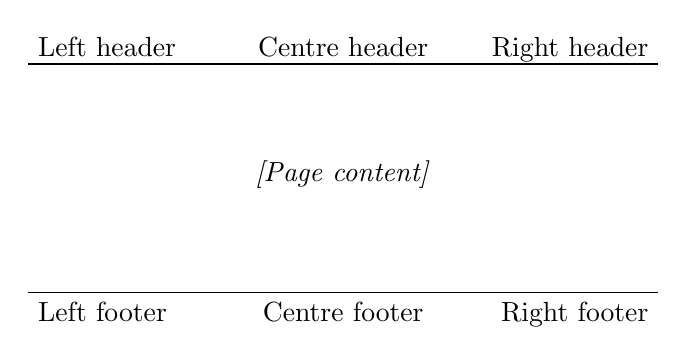
\begin{tikzpicture}
\draw (0,0) node[anchor=base west] {Left header};
\draw (4,0) node[anchor=base] {Centre header};
\draw (8,0) node[anchor=base east] {Right header};

\draw (0,-0.1)--(8,-0.1);
\draw (0,-3)--(8,-3);
\draw (4,-1.5) node {\emph{[Page content]}};

\draw (0,-3) node[anchor=north west] {Left footer};
\draw (4,-3) node[anchor=north] {Centre footer};
\draw (8,-3) node[anchor=north east] {Right footer};
\end{tikzpicture}
\end{center}

The \cmd{fancyhf} command is the basic workhorse of the package:
it takes an optional placement specifier and the header content.
The placement consists of up to three letters:
\verb|E| or \verb|O| for even and odd pages, one of \verb|LCR| for left-centre-right,
and \verb|H| or \verb|F| for header and footer.
The \cmd{fancyhead} and \cmd{fancyfoot} commands imply the header/footer specifier.

These are maybe best illustrated by an example:
%
\begin{ExampleCode}
\pagestyle{fancy}

% No specifier, so the command applies to all positions
% This clears any pre-existing content
\fancyhf[]{}

% Page number to the centre footer of all pages
\fancyfoot[C]{\thepage}

% Some text to the margin-side header
% (Left on even pages, right on odd pages)
\fancyhead[LE, RO]{\textbf{An important document}}
\end{ExampleCode}

To access the current chapter and section name,
you can use the marks described in \Cref{sec:marking}.
The following code replicates the default \LaTeX{} \verb|headings| page style:
%
\begin{ExampleCode}
\pagestyle{fancy}

% Clear all
\fancyhf[]{}

% Page number to outer edge
\fancyhead[LE,RO]{\thepage}

% Mark to inner edge
\fancyhead[RE]{\leftmark}
\fancyhead[LO]{\rightmark}
\end{ExampleCode}


\begin{remark}
The package gives a warning if the header height is not large enough.
The warning even gives a suggested value for the \cmd{headheight} length,
which you can pass to \pkg{geometry} (or do a raw \verb|\setlength|, if not using the package).
\end{remark}

You can customize the rule separating header and text by redefining the
\cmd{headrulewidth} length, and correspondinly \cmd{footrulewidth}.
It is also possible to customize the separation from header text and the line style,
but for these we refer to the package documentation.%
\footnote{One has to be a bit careful with vertical spacing.}

\chapter{Mathematics layout}\label{sec:mathematics}

Plain \TeX{} already provides a lot of facilities for typesetting mathematics,
and this is further extended by \LaTeX{} and the \pkg{amsmath} packages.
The \pkg{amsmath} package is essentially as old as \LaTeX{}.
It is automatically loaded by the Americal Mathematical Society document classes like \verb|amsart|,
so you might not even need to load it.

The package works well but has not been significantly updated since the nineties.
Some additions and bug fixes are collected in the \pkg{mathtools} package.
If you use a non-AMS document class, you can load \pkg{mathtools} instead of \pkg{amsmath}
to get slightly improved typesetting.

\begin{technote}
The \pkg{amsmath} package used to be tied to the AMS document classes,
but it is nowadays maintained by the \LaTeX{} core team.
It is one of the packages guaranteed to be present on every \LaTeX{} distribution.
\end{technote}


%
%
%
\section{Equation environments}

Standard \LaTeX{} provides the \verb|\[ ... \]| syntax for
creating a mathematics display (as opposed to inline mathematics with \verb|$ ... $|).
This environment does not support equation numbering or line breaks;
for those, \pkg{amsmath} provides a lot of options.

\begin{warning}
Plain \TeX{} used the \verb|$$ ... $$| syntax for display mathematics.
Do not use it -- the \LaTeX-style environment has some hooks and accessibility features
that the \TeX{} syntax does not have.
\end{warning}


%
%
\subsection{Single numbered equation}

The basic equation environment of \pkg{amsmath} is \env{equation}.
It sets its contents on a single line and numbers the equation:
%
\begin{VerbatimOut}{\jobname.tmp}
\begin{equation}
i \partial_t u - \Delta u = -u^3.
\end{equation}
\end{VerbatimOut}
\ShowExample

If you'd rather have an unnumbered equation,
you can use the \verb|equation*| environment.
It is essentially equivalent to \verb|\[ \]| of \LaTeX.

To customize the equation number, you can use the \cmd{tag} command.
%
\begin{VerbatimOut}{\jobname.tmp}
\begin{equation}
i \partial_t u - \Delta u = -u^3.
\tag{NLS}
\end{equation}
\end{VerbatimOut}
\ShowExample
%
The tag also appears in cross-references to this equation.
The tag is read in text mode, so any mathematical symbols need to be wrapped with \verb|$|.

If you want to change whether equations are numbered globally or per section,
use the \cmd{numberwithin} mechanism described in \Cref{sec:counters}:
%
\begin{ExampleCode}
\numberwithin{equation}{section}
\end{ExampleCode}


%
%
\subsection{Single equation on many lines}

You can break a long expression into multiple lines with the \env{multline} environment.
Only one equation number is produced (none if you use \verb|multline*|).
Line breaks are specified with \verb|\\|:
%
\begin{VerbatimOut}{\jobname.tmp}
\begin{multline}
a^5 + 5 a^4 b \\
+ 10 a^3 b^2 + 10 a^2 b^3\\
+ 5 a b^4 + b^5
\end{multline}
\end{VerbatimOut}
\ShowExample
%
The first line is left-aligned, the last line is right-aligned,
and the rest are centered.

If you need to control the alignment,
you can use the \env{split} environment.
This environment needs to be put inside \verb|equation| (or \verb|equation*|).
The alignment point is denoted by \verb|&|:
%
\begin{VerbatimOut}{\jobname.tmp}
\begin{equation}
\begin{split}
(a+b)^2
&= (a+b)(a+b)\\
&= a^2 + 2ab + b^2.
\end{split}
\end{equation}
\end{VerbatimOut}
\ShowExample

Sometimes, you need to align with things that are not really there.
Let us produce a slightly different version of the previous example:
%
\begin{VerbatimOut}{\jobname.tmp}
\begin{equation}
\begin{split}
&\mathrel{\phantom{=}} (a+b)^2\\
&= (a+b)(a+b)\\
&= a^2 + 2ab + b^2.
\end{split}
\end{equation}
\end{VerbatimOut}
\ShowExample
%
The \cmd{phantom} command reserves enough space on the first line for $=$,
even though it is not printed there;
the \cmd{mathrel} command ensures that the spacing is that surrounding $=$ as well.
This ensures that the expressions are aligned.
The same effect can not be attained with moving the alignment symbol,
since the \TeX{} spacing algorithm (described below) cannot see across the \verb|&|:
%
\begin{VerbatimOut}{\jobname.tmp}
Bad spacing after $=$ sign:
\begin{equation}
\begin{split}
&(a+b)^2\\
= &(a+b)(a+b)\\
= &a^2 + 2ab + b^2.
\end{split}
\end{equation}
\end{VerbatimOut}
\ShowExample



%
%
\subsection{Many equations, many lines}

The \env{gather} environment collects equations, each centered.
%
\begin{VerbatimOut}{\jobname.tmp}
\begin{gather}
(a+b)^2 = a^2 + 2ab + b^2,\\
a^2 - b^2 = (a+b)(a-b).
\end{gather}
\end{VerbatimOut}
\ShowExample

This environment also supports \env{split} on one or more sub-equations:
%
\begin{VerbatimOut}{\jobname.tmp}
\begin{gather}
(a+b)^2 = a^2 + 2ab + b^2,\\
\begin{split}
(a+b)^3 &= a^3\\
&\mathrel{\phantom{=}} + 3a^2 b + 3ab^2 + b^3.
\end{split}
\end{gather}
\end{VerbatimOut}
\ShowExampleBelow

You can customize the tag of each individual equation with \cmd{tag},
and also suppress an individual tag with \cmd{notag}.
These commands can appear anywhere before the \verb|\\| that ends the particular equation.
Again, the \verb|gather*| environment suppresses all tags
except those explicitly created with \cmd{tag}.
%
\begin{VerbatimOut}{\jobname.tmp}
\begin{gather}
(a+b)^2 = a^2 + 2ab + b^2,\\
(a+b)^3 = a^3 + 3a^2 b + 3a b^2 + b^3, \notag\\
a^2 - b^2 = (a+b)(a-b). \tag{$\ast$}
\end{gather}
\end{VerbatimOut}
\ShowExampleBelow

If you need to have several aligned equations, you can use the \env{align} environment.
In comparison to \env{split}, each line is now numbered individually:
%
\begin{VerbatimOut}{\jobname.tmp}
\begin{align}
(a+b)^2
&= (a+b)(a+b)\\
&= a^2 + 2ab + b^2.
\end{align}
\end{VerbatimOut}
\ShowExample
The same remarks about \cmd{tag} and \cmd{notag} with \verb|gather| apply here.
The \env{align} environment also supports more than one alignment point.


\begin{warning}
There is also an \obsenv{eqnarray} environment provided by base \LaTeX.
It is far less sophisticated and generally uglier than
anything you can achieve with the environments presented here,
so I would avoid it.
\end{warning}

If you want to number the equations as subequations,
it can be done by wrapping the environment inside \env{subequations}:
%
\begin{VerbatimOut}{\jobname.tmp}
\begin{subequations}  
  \begin{align}
    (a+b)^2
    &= (a+b)(a+b)\\
    &= a^2 + 2ab + b^2.
  \end{align}
\end{subequations}
\end{VerbatimOut}
\ShowExample


If your equation environment is very long,
it might be beneficial to allow page breaks.
The display environments presented here do not allow page breaks by default.
By putting a \cmd{displaybreak} command before the \verb|\\|,
you indicate that a page break \emph{is allowed}.

The \cmd{allowdisplaybreaks} command permits page breaks in displays everywhere in its scope.
If you put it inside an environment, it applies to that environment only;
if you put it in the preamble, it applies to all environments.


%
%
\subsection{Cases}

To group several expressions with vertical brackets,
you can use the \env{cases} environment inside an equation environment.
This environment supports a single alignment \verb|&|:
%
\begin{VerbatimOut}{\jobname.tmp}
\begin{equation}
f(n) = \begin{cases}
    n^2, & n > 0,\\
    -n, & n \leq 0.
\end{cases}
\end{equation}
\end{VerbatimOut}
\ShowExample
%
If you mostly have text following the alignment character,
you can use the starred environment.
It interprets the right-hand side of \verb|&| in text mode:
%
\begin{VerbatimOut}{\jobname.tmp}
\begin{equation}
f(n) = \begin{cases*}
    n^2+1, & if $n$ is even,\\
    n+7, & if $n$ is odd.
\end{cases*}
\end{equation}
\end{VerbatimOut}
\ShowExample

They also have a right-aligned cousin \env{rcases}:
%
\begin{VerbatimOut}{\jobname.tmp}
\begin{equation}
\begin{rcases}
i \partial_t u - \Delta u = -u^3,\\
\partial_{tt} u - \Delta u = -u^3
\end{rcases}
\text{ some dispersive PDE}
\end{equation}
\end{VerbatimOut}
\ShowExampleBelow

If you want to number lines in the \verb|cases| environment individually,
check out the \pkg{cases} package.


%
%
\subsection{Matrices}

Like \verb|cases|, matrices are not equation environments on their own,
but can appear inside one.
There are a few variants depending on how you like them:
%
\begin{VerbatimOut}{\jobname.tmp}
\begin{gather*}
\begin{pmatrix}
    1 & 2\\
    3 & 4
\end{pmatrix}\\
\begin{bmatrix}
    1 & \cdots & 1\\
    0 & \ddots & \vdots\\
      & \cdots & 1
\end{bmatrix}\\
\begin{vmatrix}
    a & b\\
    c & d
\end{vmatrix}
\end{gather*}
\end{VerbatimOut}
\ShowExample




%
%
%
\section{Fonts and text in mathematics}

In mathematical mode \TeX{} follows different spacing rules.
Spaces are ignored, and the spacing between letters is slightly altered:
%
\begin{VerbatimOut}{\jobname.tmp}
\emph{some text}\\
$some text$
\end{VerbatimOut}
\ShowExample
%
\todo{Subscript stat}
You should never write operators like $\sin$ with \verb|\mathrm|;
see \Cref{sec:operators} for the correct way to do them.

\begin{practices}
Also the spacing of punctuation is slightly different in math mode.
You should use math mode only for mathematics;
in particular, the second example below is preferable:
%
\begin{VerbatimOut}{\jobname.tmp}
Summing over $i, j, k$, we find\dots\\
Summing over $i$, $j$, $k$, we find\dots\\
\end{VerbatimOut}
\ShowExample
\end{practices}

To put text inside a math display, use the \cmd{text} command of \pkg{amsmath}.
Since spaces are ignored in math mode, you need to put the spacing inside the argument.
(Quite often, it is useful to add a bit more space with the manual spacing commands described below.)
%
\begin{VerbatimOut}{\jobname.tmp}
\[
a_k < a_{k+1}
\text{ for all } k \in \mathbb N.
\]
\end{VerbatimOut}
\ShowExample
%
The argument inside \cmd{text} is interpreted in text mode,
but it is in fact possible to enter math mode again with \verb|$|:
%
\begin{VerbatimOut}{\jobname.tmp}
\[
a_k < a_{k+1}
\text{ for all $k \in \mathbb N$, and }
a_1 > 1.
\]
\end{VerbatimOut}
\ShowExampleBelow

Inside an \env{align} environment, you can do short interjections with \cmd{intertext}.
\todo{intertext}

\begin{practices}
Do not overuse \cmd{intertext}.
It is suitable only for short notes.
\end{practices}

\todo{amsfonts}


%
%
%
\section{Mathematical symbols and whitespace}

\LaTeX{} and \pkg{mathtools} already provide quite a lot of symbols,
but if those are not enough, there are many extension packages.
The first two to consider are \pkg{amssymb} (AMS symbol font)
and \pkg{stmaryrd}.
There are also some specialized packages like \pkg{braket} for Dirac bra-ket notation.

\begin{gotcha}
The \pkg{stmaryrd} package should be loaded \emph{after} \pkg{amssymb},
since it extends and modifies some symbols there.
\end{gotcha}

If you're not interested in browsing through package documentation to find symbols,
the Detexify tool\footnote{\url{detexify.kirelabs.org}} is your friend.\index{Detexify}\index{symbols!finding}
You can draw the symbol in this web app,
and it searches for it in \LaTeX{} symbol list and a large collection of extension packages.%
\footnote{\url{www.ctan.org/tex-archive/info/symbols/comprehensive}
is your friend if you want to search manually;
be advised that this PDF is over 30~MB and almost 500~pages in size.}


%
%
\subsection{Spacing}

\TeX{} is quite smart about figuring out the spacing between different mathematical symbols.
Just look at the difference between $2 - 1$ and $2 (-1)$.
Sometimes, it is important to choose the command properly to get expected spacing.
Compare the two examples:
%
\begin{VerbatimOut}{\jobname.tmp}
$f : A \to B$\\
$f \colon A \to B$
\end{VerbatimOut}
\ShowExample

Let us first see the manual commands for spacing,
since their sizes correspond to units used by \TeX.
Note that the difference of the units is very small,
just enough to be perceptible:
These commands can be used to manually tweak spacings.
However, even better is to let \TeX{} automate things.

Internally, every mathematical symbol belongs to a symbol class.\index{symbol classes}
These are listed in \Cref{tbl:math symbol classes}.
\TeX{} puts a space between two symbols based on their respective classes.
For example, there is no space between two ordinary characters,
whereas there is a medium \verb|\:| space between binary and ordinary symbols.

\begin{table}
\centering
\begin{tabular}{l|cc}
Symbol class & Override command & Examples\\
\hline
Ordinary & \cmd{mathord} & $2 x$\\
Operator & \cmd{mathop} & $\sin$\\
Binary & \cmd{mathbin} & $2 + x$\\
Relation & \cmd{mathrel} & $2 < x$\\
Opening & \cmd{mathopen} & $( \quad \lfloor$\\
Closing & \cmd{mathclose} & $) \quad \rfloor$\\
Punctuation & \cmd{mathpunct} & $,$
\end{tabular}
\caption{The mathematical symbol classes.}
\label{tbl:math symbol classes}
\end{table}

We talk more about operators below in \Cref{sec:operators},
so let us consider binary operations as our example.
Usually $\heartsuit$ is considered an ordinary symbol,
but let us imagine that we have defined it as an operation between two expressions.
Then it would be necessary to wrap its use in \cmd{mathbin} in order to get correct spacing.
\todo{DeclareMathSymbol}
%
\begin{VerbatimOut}{\jobname.tmp}
\newcommand{\friends}{\mathbin\heartsuit}

Bad: $x \heartsuit y$\\
Good: $x \friends y$.
\end{VerbatimOut}
\ShowExample
%
Some combinations of symbol classes are considered impossible,
in which case \TeX{} modifies one of the classes suitably.
To go back to the example of the minus sign,
\verb|-| is usually defined as a Relation symbol.
However, if it is not preceded by an Ordinary symbol (like a number),
it is transformed into Ordinary itself -- this means that \verb|-1| produces no spacing at all.

\begin{gotcha}
This somewhat explains the difference between \verb|:| and \cmd[spacing]{colon}, but only partly.
The symbol \verb|:| is classified as Relation and \cmd[spacing]{colon} as Punctuation.
However, \pkg[colon]{amsmath} further modifies the spacing of \cmd[spacing]{colon}
to fit the $f \colon A \to B$ pattern -- and only that pattern.

If you ever need the colon as a punctuation symbol, you can wrap it in \verb|\mathpunct{:}|.
\end{gotcha}

\begin{gotcha}
Another source of confusion is \verb.|. and \cmd[spacing]{mid}.
The first is Ordinary and the second Relation.
They should be used correspondingly:
\verb.|a|. for the absolute value $|a|$,
\verb.f|_A. for the restriction of a function $f|_A$,
and \verb.a \mid b. for the divisibility relation $a \mid b$.
\end{gotcha}

\begin{gotcha}
The symbols \verb|. ! ?| are of class Ordinary, not Punctuation.
This is to do with their mathematical meanings.
\end{gotcha}

\begin{gotcha}
Adding an accent turns the symbol into Ordinary.
%
\begin{VerbatimOut}{\jobname.tmp}
$a \hat= b$\\
$a \mathrel{\hat=} b$
\end{VerbatimOut}
\ShowExample
\end{gotcha}

\begin{gotcha}
The occasionally used notation for open intervals conflicts with the algorithm,
since \verb|]a, b[| is understood as Closing--Opening pair instead of the opposite.
It can be fixed manually as in the next example:
%
\begin{VerbatimOut}{\jobname.tmp}
$f \colon ]a, b[ \to ]0, 1]$\\
$f \colon \mathopen]a, b\mathclose[
    \to \mathopen]0, 1]$
\end{VerbatimOut}
\ShowExample
%
A quick fix is to wrap the intervals inside \verb|{}|.
If you use a lot of intervals,
you should either define some custom commands or check out the \pkg{interval} package.
\end{gotcha}



One common pain point is the humble $\mathrm dx$ that appears in integrals.
It is nice to get the spacing consistently right,
and note also the upright $\mathrm d$ (this is advocated by an ISO standard, but some prefer $dx$).
\index{dx@$\mathrm dx$}

A common way to do this (based on Stack Exchange discussions) is:
%
\begin{VerbatimOut}{\jobname.tmp}
\newcommand{\diff}{\mathop{}\!\mathrm{d}}

In an integral:
\[
\int_0^1 x \diff x,
\]
and inside parens: $\mu(\diff x)$.
\end{VerbatimOut}
\ShowExample
%
Note the automatic space between $x$ and $\mathrm dx$.

What happens here is that the empty group \verb|{}| is set in operator style.
When preceded by an ordinary symbol, the operator style puts a thin \verb|\,| space;
when preceded by punctuation like \verb|(|, the space is not present.
The thin \verb|\,| space between the (empty) operator and `d' is cancelled with \verb|\!|.

If you find yourself writing lots of complicated differentials like
\[
\frac{\mathrm d^2 \log(x)}{\mathrm dx^2},
\]
you should look into the \pkg{diffcoeff} package
that provides a slightly shorter syntax.


%
%
\subsection{Operators and limits}\label{sec:operators}
One common class of text in mathematics is operators.
Compare the three examples here:
%
\begin{VerbatimOut}{\jobname.tmp}
Awful: $2 sin \pi$,\\
Still bad: $2 \textrm{sin} \pi$,\\
Good: $2 \sin \pi$.
\end{VerbatimOut}
\ShowExample
Here the \verb|\sin| command not only sets the operator name properly,
but also adjusts the spacing around the operator.

If the operator you need is not predefined as a \LaTeX{} command,
you can do the styling once with \cmd{operatorname}\dots
%
\begin{VerbatimOut}{\jobname.tmp}
\[
2 \operatorname{dim} X
\]
\end{VerbatimOut}
\ShowExample
%
\dots{}or define a new command with \cmd{DeclareMathOperator} in the preamble:
%
\begin{VerbatimOut}{\jobname.tmp}
% In the preamble:
% \DeclareMathOperator{\arccosh}{arccosh}

\[
2 \arccosh \pi
\]
\end{VerbatimOut}
\ShowExample

For certain operators, limits can be put either to the side or above/below the operator.
Compare these two:
\[
\text{text style }\textstyle \sum_{i=1}^\infty
\text{ and display style }\displaystyle \sum_{i=1}^\infty.
\]
There are package options to \pkg{amsmath}/\pkg{mathtools}
to control how the limits are placed in display equations.
By default, they are placed on the side for integrals and above/below for everything else.

To put limits above/below your custom operator, use the starred form of the declaration:
%
\begin{VerbatimOut}{\jobname.tmp}
\[
\operatorname{dim}_H^\ast X
\text{ vs }
\operatorname*{dim}_H^\ast X
\]
\end{VerbatimOut}
\ShowExample

If you need to put multiple lines of text in a sum argument,
you can use the \cmd{substack} command.
Inside its argument, you can use the usual \verb|\\| line breaks:
%
\begin{VerbatimOut}{\jobname.tmp}
\[
\sum_{\substack{1 \leq j \leq 10\\ 1 \leq k \leq j}}
\]
\end{VerbatimOut}
\ShowExample

\todo{mathtools offers cramped versions}

Some special operators that deserve a mention are the modulus operators,
since they have some special spacing rules:
%
\begin{VerbatimOut}{\jobname.tmp}
\begin{gather*}
a \equiv b \mod p\\
a \equiv b \bmod p\\
a \equiv b \pmod p
\end{gather*}
\end{VerbatimOut}
\ShowExample


%
%
\subsection{Fractions}
There are two basic fraction-like commands: \cmd{frac} for fractions,
and \cmd{binom} for binomial coefficients.
Both take the numerator and denominator as their arguments.

To produce generalized fraction-like operators like
\[
\genfrac{(}{)}{}{}{a}{b}
\quad\text{and}\quad
\genfrac{\lfloor}{\rceil}{0pt}{}{a}{b},
\]
the \pkg{amsmath} package provides the \cmd{genfrac} command.
Read the package documentation to understand its six parameters.

Continued fractions are produced with the \cmd{cfrac} command:
%
\begin{VerbatimOut}{\jobname.tmp}
\[
\cfrac{1}{\sqrt 3 + \cfrac{2}{\sqrt 3 + \dotsb}}
\]
\end{VerbatimOut}
\ShowExample

\begin{warning}
Plain \TeX{} does fractions and binomials with the \obscmd{over} and \obscmd{choose} commands
that have a different syntax: \verb|n \choose m| instead of \verb|\binom n m|.
As natural as the syntax might seem, you should only use the \LaTeX{} constructs.
\end{warning}


%
%
\subsection{Building new symbols}

\todo{Shortly on this}

\todo{Negations}



%
%
%
\section{Size in mathematics}

Delimiting symbols come in five sizes:
\begin{VerbatimOut}{\jobname.tmp}
\[
( \big( \Big( \bigg( \Bigg(
\]
\end{VerbatimOut}
\ShowExample
%
Instead of setting the size manually,
the \cmd{left} and \cmd{right} commands can be used.
They choose the size based on the content between delimiters.
Accordingly, the two commands must be paired correctly.
There is also \cmd{middle} for an optional middle delimiter in the matching size.
%
\begin{VerbatimOut}{\jobname.tmp}
\[
\left\{ a \in \mathbb Q
  \middle| a^2 < \frac 1 2 \right\}
\]
\end{VerbatimOut}
\ShowExample

\begin{gotcha}
It is not possible to have a line break between \cmd{left} and \cmd{right},
so in long formulas you might need to do the sizing manually.
\end{gotcha}

\begin{practices}
I like to define the following two commands in my documents:
%
\begin{VerbatimOut}{\jobname.tmp}
\newcommand{\abs}[1]{\left|#1\right|}
\newcommand{\norm}[1]{\left\|#1\right\|}

Absolute value $\abs x$,\\
function norm $\norm f$.
\end{VerbatimOut}
\ShowExample
%
They are both semantically meaningful and automatically sized.
\end{practices}

There are two basic styles of sizing other mathematics: text style and display style
(there are also two levels of sub-/superscript styles).
The first is used with inline mathematics and the latter with display mathematics.
It is possible to override the style with \cmd{textstyle} and \cmd{displaystyle}:
%
\begin{VerbatimOut}{\jobname.tmp}
Text with oversize
$\displaystyle \binom n m \frac 1 2$
mathematics, and a display with small maths:
\[
\sqrt{\textstyle \binom n m \frac 1 2}
\]
\end{VerbatimOut}
\ShowExample
%
For fractions, there are the abbreviated \cmd{tfrac} and \cmd{dfrac} commands
to achieve this effect.


%
%
%
\section{Decorations}

\subsection{Accents}

You should not use accented Unicode characters like `â' in math mode.
Instead, write \verb|\hat a|.
The supported accents are listed in various places online.%
\footnote{\url{https://en.wikibooks.org/wiki/LaTeX/Mathematics\#Accents}}

\begin{gotcha}
The accents apply to the immediately succeeding character,
and do not take subscripts into account.
Compare the three:
%
\begin{VerbatimOut}{\jobname.tmp}
$\hat a_0$ vs $\hat {a_0}$
vs $\widehat {a_0}$
\end{VerbatimOut}
\ShowExample
\end{gotcha}

To put material over and under symbols,
there are the aptly named \cmd{overset}, \cmd{underset}, and \cmd{overunderset} commands:
%
\begin{VerbatimOut}{\jobname.tmp}
\[
\overset{\eqref{eq:pythagoras}}{=}
\quad \underset{\ast}{X}
\quad \overunderset{a}{b}{C}
\]
\end{VerbatimOut}
\ShowExample
%
To produce some very cursed versions of big operators,
there is also the \cmd{sideset} command:
%
\begin{VerbatimOut}{\jobname.tmp}
\[
\sideset{^a_b}{^c_d}\sum_{i=1}^\infty
\]
\end{VerbatimOut}
\ShowExample



%
%
\subsection{Dots}

The \pkg{amsmath} package provides a context-sensitive \cmd{dots} command.
Compare the vertical positions of the dots in these two examples:
%
Thanks to this, is is usually enough to use \cmd{dots} everywhere in your mathematics.
The exception is at the end of expression,
since \pkg{amsmath} decides the placement by looking at the following symbol.
You can give a hint with commands like \verb|\dotsc| (dots with commas)
and \verb|\dotsb| (dots with binary operations)
and even \verb|\dotsi| (dots with integrals) for these cases.

Of course, if memorizing these seems too much, the usual \verb|\cdots| and \verb|\ldots| can be used;
they just tie the semantics and presentation together.


%
%
\subsection{Braces and highlighting}
There are two commands for producing horizontal braces:
\cmd{overbrace} and \cmd{underbrace}.
They both accept explanatory text as super-/subscript respectively.
%
\begin{VerbatimOut}{\jobname.tmp}
\[
\overbrace{a^2 + b^2}^{\text{catheti}}
= \underbrace{c^2}_{> 0}.
\]
\end{VerbatimOut}
\ShowExample

The \pkg{mathtools} package also provides similar commands for brackets.
They can be optionally customized in thickness and height,
but they do not support text:
%
\begin{VerbatimOut}{\jobname.tmp}
\[
\overbracket[1pt][0.5cm]{a^2 + b^2}
= \underbracket[3pt]{c^2}.
\]
\end{VerbatimOut}
\ShowExample

Relatedly, let us just note that \pkg{amsmath} provides a \cmd{boxed} command
for drawing a box around some mathematics.
If the argument continues across a \verb|&| alignment point,
you need the \pkg{mathtools} variant \cmd{Aboxed}.
A more extensible version is provided by the \pkg{empheq} package.
%
\begin{VerbatimOut}{\jobname.tmp}
\[
\boxed{a^2 + b^2} = c^2.
\]
\end{VerbatimOut}
\ShowExample

If you want to emphasize something with colour,
the \pkg{xcolor} package offers a \cmd{mathcolor} command that works
just like its text counterpart:%
\footnote{To be precise, it works \emph{very much unlike} its text counterpart in that
if you try to use \texttt{\textbackslash textcolor} in math mode, it breaks the spacing.}
%
\begin{VerbatimOut}{\jobname.tmp}
\[
\mathcolor{blue}{a^2 + b^2} = c^2.
\]
\end{VerbatimOut}
\ShowExample


%
%
\subsection{Arrows}
Mathematicians seem to like arrows.\index{arrows!mathematics}
Here is a sample of some;
note that some have synonyms for semantically more meaningful code.
You probably can deduce the rules for even further variants:
\begin{VerbatimOut}{\jobname.tmp}
\begin{gather*}
\gets \to \mapsto\\
\leftarrow \uparrow \nwarrow \searrow \rightarrow\\
\Leftarrow \Leftrightarrow \Rightarrow\\
\Longleftarrow \Longleftrightarrow \implies\\
\hookleftarrow \rightharpoonup\\
\leftrightharpoons \rightleftharpoons
\end{gather*}
\end{VerbatimOut}
\ShowExample

Sometimes it is useful to put longer sub- or superscripts on arrows.
The \pkg{amsmath} package provides extensible versions of arrows.
The command names are prefixed with \verb|x|,
and the optional argument goes below and the main argument above the arrow:
%
\begin{VerbatimOut}{\jobname.tmp}
\begin{gather*}
f(x) \xrightarrow[n \to \infty]{\text{weakly}} 0\\
b^2 = 0
\xRightarrow{\eqref{eq:pythagoras}} a^2 = c^2
\end{gather*}
\end{VerbatimOut}
\ShowExample

\begin{gotcha}
These extended arrows should only be used in display size.
\end{gotcha}

While we are on the topic of arrows,
let us mention the commutative diagrams that are popular among some mathematicians.
For simple diagrams the \pkg{amscd} package by AMS provides a terse syntax;
for more complicated diagrams there is \pkg{tikz-cd} based on TikZ.



%
%
%
\section{Theorem environments}

\todo{Putting QED where it belongs (and customizing it)}

\chapter{Tools for serious publications}

\section{Cross-references and hyperlinks}

\section{Bibliography management}\label{sec:bibliography}

\section{Table of contents}

\chapter{Further customization}

\section{Alternative \LaTeX{} compilers}

During the years, the preferred output format of \TeX{} has changed:
\begin{enumerate}
\item The original implementation of \TeX{} produced DVI~files
    -- this was a device-independent format that could be processed into commands
    to be sent to the printer or photo\-type\-setting machine.
\item Simultaneously in the 1980s, Adobe developed the PostScript format.
    PostScript is a language for expressing complex drawing commands to printers.%
\footnote{Processing drawing commands requires processing power and memory.
The original Apple laser printers were \emph{more powerful} than the
Macintosh computers used to lay out the documents!}
    It became the universal standard,
    and in the 1990s a lot of \TeX{} documents were put online as \verb|.ps| files.
    These files were produced from DVI~files by a converter.
\item PDF (Portable Document Format), also by Adobe,
    was created in the 1990s and has become the dominant standard.
    PDF encapsulates a subset of PostScript, image data, and metadata about the document.
\end{enumerate}

Originally, PDF~files were produced by first converting DVI to PostScript and then to PDF.
In early 2000s, a new implementation of \TeX{} appeared: \prg{pdftex}.
It produces PDF~files directly and supports some special features of the format:
For example, the \pkg{pdflscape} package can tell the PDF reader
to display a landscape page in rotated mode.

\begin{technote}
The only difference between \textbf{pdftex} and \textbf{pdflatex}
is whether the \LaTeX{} macros are automatically loaded.
These notes make no effort at being consistent with the names.
\end{technote}


Another development was with the character sets.
Original \TeX{} used 7~bits per character, because 128~characters is enough for anybody
(that is, anybody writing in English).
In the 1980s, this was recognized as unsustainable,
so the character set was \emph{doubled} into 8~bits.
Any further extensions to that are based on swapping fonts on the fly.

This limitation applies also to \prg{pdftex},
but in the current\footnote{Read: past 20~years.} age of Unicode there are now alternatives.
The two major alternative compilers are
\begin{itemize}
\item \prg{luatex}, which is based on \prg{pdftex} source code.
    It uses Unicode as its native character set.
    As the name suggests, extension packages can be also written in the Lua programming language.
    Some packages like TikZ use the Lua support for a speed boost.
\item \prg{xetex} is an independent Unicode-native development
    that uses a completely different PDF backend.
    It produces a bit smaller PDF files than \prg{luatex},
    but it is less actively maintained.
\end{itemize}

Both of these ``modern'' engines support loading arbitrary OpenType fonts
with the \pkg{fontspec} package, unlike \prg{pdftex}.
(This is discussed in \Cref{sec:typefaces}.)
The native use of Unicode also means that letters like `ä'
really are output as the glyph `ä',
not \texttt{\textasciidieresis a} superimposed on top of each other
-- something you only see when copying text from a PDF~file.

\begin{practices}
Based on the discussion above,
it would be natural to suggest always using \prg{luatex}.
For personal writing, either of the Unicode engines should be the first choice.

Alas, arXiv and many publishers still use \prg{pdftex} in their pipeline.
This means that we are still stuck with making our articles \prg{pdftex}-compatible.
Hopefully the situation will change soon enough.
\end{practices}



%
%
%
\section{Accessibility of documents}

The PDF file format is principally a set of instructions to a printer:
draw a curve here, another there, and so on.
This poses a problem for accessibility.
Some examples of accessibility issues are:
%
\begin{itemize}
\item Can a ``screen reader'' program read the document aloud for a blind person?
\item Can a visually impaired person increase the color contrast on graphics?
\item Can the text from the document be copy-pasted into another program?
\end{itemize}
%
Note that the last point might not sound like an accessibility issue,
but it is caused and solvable by the same reasons.

There are three layers of accessibility work going on:
%
\begin{enumerate}
\item The PDF format can include semantic metadata about the document contents.
    \LaTeX{} is increasingly better at writing this metadata,
    but it might require you to opt in to the new behavior.
\item \LaTeX{} can be compiled into another format, such as HTML web page.
    This approach is increasingly used by major publishers and arXiv.
    It requires you to use a sensible subset of \LaTeX.
\item Source code is very accessible to a screen reader program;
    a well-written \verb|.tex| file is a good workaround.
    This still requires you to write clean code.
\end{enumerate}
%
We will briefly explore each of these layers below.

\begin{practices}
Accessibility is for everybody.
Most people benefit from some accommodations at some point in their life.
Even without an ``obvious'' disability, think about reading your document
\begin{itemize}
    \item on an ebook reader with grayscale screen (visual impairment),
    \item on a mobile phone in bright sunlight (ditto), or
    \item by a sleep-deprived parent between meetings (cognitive impairment).
\end{itemize}
Not all accessibility issues have technological solutions
-- they also require you to think about how you present your message.
A complicated figure is hard to read, no matter the technology used to produce it.
\end{practices}


%
%
\subsection{PDF accessibility}

This is the core accessibility work done by the \LaTeX{} team during the last few years.
The goal is to embed semantic metadata about the document into the PDF format.
A lot of the semantics is in the \verb|.tex| source in form of sectioning commands and such.

The translation is hampered by the need to rewrite \LaTeX{} internals without breaking compatibility,
and all the abuse of commands to get semantically incorrect but visually good results.

To enable PDF metadata, you should do the following steps:
\begin{itemize}
\item Use a modern \LaTeX{} compiler like LuaL\prg{luatex} or \prg{xetex}.
    Since \prg{luatex} is more actively maintained, it is preferable.
\item Add \cmd{DocumentMetadata} as the first line (before \verb|\documentclass|) of the code.
\item Load the \pkg{hyperref} package.
\item Consider loading the \pkg{unicode-math} package
    (and remove other mathematics symbol and font packages;
    see page~\pageref{rem:math unicode}).
\end{itemize}

\begin{warning}
Since some behavior changes subtly,
you should take these into use only in new projects
and only when everybody involved (including the publisher) uses a Unicode-native \LaTeX{} pipeline.

Be extra careful with checking the output when converting old projects,
or if you need to compile the project with both old and new toolsets.
\end{warning}

\begin{warning}
As of April~2024, arXiv \emph{does not} use Unicode-native \LaTeX{} tools;
their process involves \prg{pdftex}.
For arXiv submissions, follow the next section instead.
\end{warning}

The \cmd{DocumentMetadata} command tells \LaTeX{} that you opt in
to new and rewritten behaviors.
For example, it enables some new features in the \pkg[opt-in features]{hyperref} package.

\begin{latexthree}
This work is still heavily in progress.
There are some arguments to \cmd{DocumentMetadata} that enable further in-development features.
As of April~2024 these include tagging of mathematics and tables.

Since these arguments are unstable, they are not documented here
and should not be used in ``real'' documents quite yet.
You can follow the progress through \LaTeX{} release newsletters:
\begin{quote}
\url{https://www.latex-project.org/news/}
\end{quote}
\end{latexthree}

In order for the tagging to work,
you need to produce semantically correct code.
That is, use \verb|\subsection*| when you need an unnumbered subsection,
and only then -- do not abuse it for bold, heavy text.
Similarly, use \verb|\emph| to emphasize,
instead of \verb|\textit| or \verb|\textbf| that carry only visual meaning.


%
%
\subsection{HTML conversion}

Another option is to skip PDF altogether.
The most common alternative format is HTML, the technology behind web pages.
It has a few benefits:
%
\begin{itemize}
\item It is processed on the user device, so e.g.\ colours can be customized by the reader.
\item The text can be reflowed based on the screen size and magnification factor.
\item Existing screen reader programs can already read out web pages.
\end{itemize}
%
However, there are a few drawbacks too:
%
\begin{itemize}
\item \TeX{} is built on the model of printing on paper; it assumes a fixed layout in many places.
\item The usual \LaTeX{} compilers only produce PDF output or equivalent.
\end{itemize}

The HTML approach is now pursued by several publishers and arXiv,
together with e.g.\ American Mathematical Society.
ArXiv uses a tool called \mbox{LaTeXML}%
\footnote{\url{https://github.com/brucemiller/LaTeXML}}
that is essentially a new \TeX{} compiler that selectively reimplements some packages.

Since \LaTeX{} is already semantically focused, this works surprisingly well.
A lot of packages are already supported.
Importantly, TikZ can output its pictures also in the SVG (Scalable Vector Graphics) format
used together with HTML.\index{TikZ!accessibility}

\begin{practices}
Load and use only the packages that you really need.
Prefer mainstream packages supported by the arXiv converter.
ArXiv has a help document outlining some more best practices for HTML conversion.\footnotemark
\end{practices}
\footnotetext{\url{https://info.arxiv.org/help/submit_latex_best_practices.html}}



%
%
\subsection{Accessible source code}

Both of the above methods require you to use semantically meaningful commands:
otherwise, the automated tools are unable to do tagging/conversion.
Yet writing good semantic \LaTeX{} code is also an accessibility feature:
you can always read the source code.

\begin{remark}
Source code posted to arXiv is public and downloadable.
\end{remark}

If you want to set vectors in bold font, then do not write \verb|\mathbf| but
redefine \verb|\vec| to set vectors in bold style:
%
\begin{VerbatimOut}{\jobname.tmp}
% Preamble
\renewcommand{\vec}{\mathbf}

$\vec a$
\end{VerbatimOut}
\ShowExample
%
Now it is immediate from the source code that \verb|a| refers to a vector.
It can not be confused with other things marked with boldface.
Besides, if you change your mind about the style,
you only need to change one command in the preamble.


%
%
%
\section{Typefaces}\label{sec:typefaces}

\todo{Point sizes}
\todo{Microtypography}

\todo{Palatino and Noto with math}

\subsection{Emoji}\label{sec:emoji}

Emoji are Unicode characters, so in principle they can be included just as is in the source code.
The problem is choosing a font that can display the characters.

The \pkg{emoji} package automatically chooses an available emoji font
(that is, the output will depend on your operating system!).
It only works with recent LuaTeX (2020 or newer).
The command provides readable shorthand names for the characters (listed in documentation):
%
\begin{ExampleCode}
% Preamble
\usepackage{emoji}

% In text
\emoji{thinking-face}
\end{ExampleCode}

There is also the manual way of loading the emoji font with \pkg[emoji]{fontspec}:
%
\begin{ExampleCode}
% Preamble
\usepackage{fontspec}
\newfontfamily{\emojifont}{Noto Color Emoji}[Renderer=Harfbuzz]

% In text
{\emojifont ...}
\end{ExampleCode}
%
Here, \verb|...| should be replaced with the emoji
(not displayed here, since these notes do not have an emoji font set up!).
You need to install the emoji font or replace it by the system emoji font.
(On Windows, it is called \texttt{Segoe UI Emoji};
on macOS it is \texttt{Apple Color Emoji}.)

\begin{overleaf}
The Overleaf editor cannot handle the Unicode emoji characters as of May~2024.
If you use Overleaf, you need to use the \pkg{emoji} package.
\end{overleaf}

\begin{warning}
With the manual way, black-and-white emoji can be displayed by both XeTeX and LuaTeX,
but color emoji requires LuaTeX with the HarfBuzz renderer.
If you use \pkg[emoji]{fontspec} to load an emoji font,
you need to pass \verb|Renderer=Harfbuzz| as an optional font feature.
This option is effective only with LuaTeX.
\end{warning}

\chapter{Figures and tables}

\section{Embedding pictures}

\section{Creating tables}

\chapter{Graphics with TikZ}

There are several methods for producing line graphics in \LaTeX.
We cover here TikZ, which is quite portable across compilers and extremely versatile.
It is contained in the \pkg{tikz} package.
There are several extension libraries that are loaded with the \cmd{usetikzlibrary} command,
and moreover many other packages are built with TikZ.

TikZ has bit of a learning curve
and its documentation spreads over no less than 1321~pages (as of April~2024).
We are able to only cover the essentials here.
An unofficial web version of the manual can be accessed at \url{https://tikz.dev/}.

\begin{technote}
TikZ is an acronym for \emph{TikZ ist kein Zeichenprogramm}
-- ``TikZ is not a drawing program''.
From this we can learn two things:
\begin{itemize}
\item Many \LaTeX{} core developers come from German-speaking Europe.
\item That as useful as TikZ is,
    for complex graphics you probably should use a proper, visual graphics editor.
\end{itemize}
Of course, the the acronym is not only recursive,
but also oxymoronic, since TikZ is a program (written in the \TeX{} language)
that outputs graphics\dots
\end{technote}

\begin{technote}
Internally, TikZ consists of three layers:
compiler-specific support code for primitive drawing operations,
a core layer called PGF,
and the (relatively) user-friendly frontend called TikZ.

Due to this, you can see references to PGF scattered in various places;
for example the CTAN page for \pkg{tikz} redirects to that of \pkg{pgf}.
In practice, the two are synonymous.
\end{technote}


%
%
\section{Coordinates, nodes, and paths}

Let us begin with a very simple example:
%
\begin{VerbatimOut}{\jobname.tmp}
\begin{tikzpicture}
  \draw[->] (0,0) -- (2,0);
  \draw[->] (0,0) -- (0,2);
  \draw[dotted] (0,0) -- ({sqrt(2)}, 1);
\end{tikzpicture}
\end{VerbatimOut}
\ShowExample
%
TikZ pictures are defined inside a \env{tikzpicture} environment.
(For small pictures, there is also a \cmd{tikz} command
that takes the contents of the environment as its single argument.)
The output appears inline in text, just as with \verb|\includegraphics| and friends.

Inside this environment, there are drawing commands.
Each of these commands \emph{ends with a semicolon}.
Forget the \verb|;| and you will get an error message.

The \cmd{draw} command is the basic workhorse of TikZ.
The \verb|--| operation draws a line between the two coordinates.
Let us first look at the syntax of coordinates before going back to the optional arguments
and different operations.

There are several coordinate systems, of which I believe the next four are most common.
\begin{description}
\item[xyz] As in the example above, coordinates in this system are
    tuples or triples of numbers separated by commas.
    These are with respect to unit vectors defined in the environment options.
    By default, the $x$ and $y$ unit vectors are 1~cm long and along the usual axes.
    The $z$ axis is skewed towards the reader.
    See the example on page~\pageref{ex:tikz basis}.

    It is possible to use mathematical syntax like \verb|+|, \verb|/|, and \verb|sqrt(...)|
    to give more complicated coordinate expressions.
    You might need to wrap the calculation inside \verb|{}|.

\item[canvas] The numbers can also have units like \verb|(1cm, 20pt)|.
    In this case the coordinates are the absolute length away from canvas origin.
    It is possible to use expressions like \verb|1cm + 2pt|.
    
    These units are still not completely absolute:
    the canvas can still be scaled with an optional argument.

    \emph{Warning}: While it is technically possible to mix canvas and xyz coordinates
    inside the tuple, it is ill-advised.
    Similarly, an expression like \verb|1+2cm| is interpreted as \verb|1pt+2cm|,
    not as ``unit vector plus 1~cm to the right''.

\item[xyz polar] Polar coordinates are like \verb|(30:2)|,
    which means: 30 degrees counterclockwise, radius 2~units.

    If the $x$ and $y$ unit vectors are set to non-default values,
    the angle corresponds to a point on the ellipse specified by $x$ and $y$ vectors,
    and the resulting vector is multiplied by the radius factor.

\item[canvas polar] Here the radius has a specified unit: \verb|(30:2cm)|.
\end{description}

There are also the barycentric coordinate system (weighted average of basis vectors)
and a possibility to compute tangents of shapes.
These are covered in \cite[Section~13.2]{tikz}.

Coordinates can be given names with the \cmd{coordinate} command.
In the example below, we also use the \verb|cycle| specifier to close the loop.
%
\begin{VerbatimOut}{\jobname.tmp}
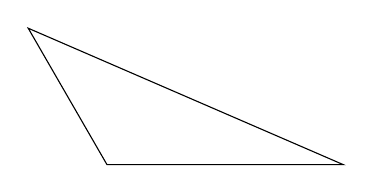
\begin{tikzpicture}
  \coordinate (A) at (0:3cm);
  \coordinate (B) at (120:2cm);

  \draw (0,0) -- (A) -- (B) -- cycle;
\end{tikzpicture}
\end{VerbatimOut}
\ShowExample

It is also possible to specify relative coordinates:
by prefixing the coordinate with \verb|++|, it is relative to the previous position.%
\footnote{It is also possible to prefix with just \texttt{+},
in which case the current position is not updated.}
%
\begin{VerbatimOut}{\jobname.tmp}
\begin{tikzpicture}
  \draw (0,0) -- ++(0:3) -- ++(90:2)
    -- ++(180:1) -- ++(270:1/2);
\end{tikzpicture}
\end{VerbatimOut}
\ShowExample


%
%
\subsection{Nodes}

Nodes can be thought of as text placed in the picture.
The text can contain mathematics and formatting commands, and even pictures.

A node can be placed either as part of a path, or separately with a \cmd{node} command.
In the latter case, it is possible to refer to the node later.
%
\begin{VerbatimOut}{\jobname.tmp}
\begin{tikzpicture}
  \draw (0,0) -- (2,0) node {Left};
  \node (A) at (0,2) {Above};
  \draw (0,0) -- (A);
  \node at (0,-1) {Below};
\end{tikzpicture}
\end{VerbatimOut}
\ShowExample

Note the difference between the lines connecting the origin to the Left and Above nodes.
When a node is created as part of a path operation,
it is \emph{centered} at the specified coordinate.
That is, the center of the ``Left'' text is at $(2,0)$.
The position of the node can be customized by passing
\verb|above|, \verb|below|, \verb|left|, or \verb|right| as an optional argument.

On the other hand, when a path is drawn to a previously defined node,
TikZ tries to stop at the boundary of the node.
It is possible to specify the position on the border by cardinal directions (like \verb|north|)
or an angle; or to specify \verb|center| if you really mean the center.
These are given by the \verb|name.anchor| syntax as in the example below.

To make the boundary of the ``Above'' node visible,
we also pass the \verb|draw| option to the \cmd{node} command.
%
\begin{VerbatimOut}{\jobname.tmp}
\begin{tikzpicture}
  \draw (0,0) -- (2,0) node[right] {Left};
  \node[draw] (A) at (0,2) {Above};
  \draw (0,0) -- (A.west);
\end{tikzpicture}
\end{VerbatimOut}
\ShowExample

One more interesting positioning specifier is the optional \verb|pos| argument.
It is understood as a position (in the range 0 to 1) on the previous path segment.
It can be combined with other specifiers as in here:
%
\begin{VerbatimOut}{\jobname.tmp}
\begin{tikzpicture}
  \draw[->] (0,0) -- (3,0)
    node[pos=0.5,above] {$\frac 1 2$}
    node[pos=0.25,below] {$\frac 1 4$}
    node[pos=0.75,below] {$\frac 3 4$};
\end{tikzpicture}
\end{VerbatimOut}
\ShowExample

To embed pictures,
you can use \cmd[in TikZ]{includegraphics} as usual inside a node.
To illustrate this once more with our fur-shedding assistants:
%
\begin{VerbatimOut}{\jobname.tmp}
\centering
\newcommand{\dogfile}{pictures/TheDogs.jpg}
\begin{tikzpicture}
  \node[draw] (Both) at (0,0)
    {\includegraphics[height=3cm]{\dogfile}};
  \node[draw] (Netta) at (-5,0)
    {\includegraphics[bb=1cm 2cm 3cm 5cm, clip, height=2cm]{\dogfile}};
  \node[draw] (Cira) at (5,0)
    {\includegraphics[bb=2.8cm 1.4cm 7cm 6cm, clip, height=2cm]{\dogfile}};
  \draw[->] (Both.west) -- (Netta.east) node[pos=0.5, above] {Netta};
  \draw[->] (Both.east) -- (Cira.west) node[pos=0.5, above] {Cira};
\end{tikzpicture}
\end{VerbatimOut}
\ShowExampleBelow[2]


%
%
\subsection{Path options}

There are lots of options that can be passed to the drawing commands.
As the very first one, let us consider \verb|color|.
It takes a colour name as its argument;
\pkg[with TikZ]{xcolor} extensions and custom colours are supported.
It is possible to blend the color with white with the \verb|!| specifier
(see page~\pageref{ex:color blending}).
Be careful with the colour name; the error message can be confusing.
%
\begin{VerbatimOut}{\jobname.tmp}
\definecolor{Sciency}{cmyk}{0,0.46,1,0}
\begin{tikzpicture}
  \draw[color=blue] (0,0)--++(3,0);
  \draw[color=LimeGreen] (0,-0.5)--++(3,0);
  \draw[color=Sciency] (0,-1)--++(3,0);
  \draw[color=Sciency!60] (0,-1.5)--++(3,0);
\end{tikzpicture}
\end{VerbatimOut}
\ShowExample

There is also a range of line weights.
Do note that their names may include spaces.
Of these, \verb|thin| is the default.
%
\begin{VerbatimOut}{\jobname.tmp}
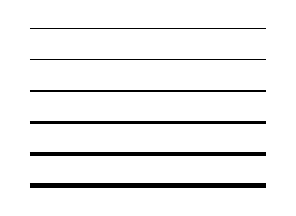
\begin{tikzpicture}[yscale=0.8]
  \draw[very thin] (0,-0.5)--++(3,0);
  \draw[thin] (0,-1)--++(3,0);
  \draw[semithick] (0,-1.5)--++(3,0);
  \draw[thick] (0,-2)--++(3,0);
  \draw[very thick] (0,-2.5)--++(3,0);
  \draw[ultra thick] (0,-3)--++(3,0);
\end{tikzpicture}
\end{VerbatimOut}
\ShowExample

Then, there are the line styles.
The basic ones are (it is possible to specify custom ones, but that you have to read from the docs):
%
\begin{VerbatimOut}{\jobname.tmp}
\begin{tikzpicture}[yscale=0.8]
  \draw[solid] (0,0.5)--++(3,0);
  \draw[dashed] (0,-0)--++(3,0);
  \draw[dotted] (0,-0.5)--++(3,0);
  \draw[densely dashed] (0,-1)--++(3,0);
  \draw[densely dotted] (0,-1.5)--++(3,0);
  \draw[loosely dashed] (0,-2)--++(3,0);
  \draw[loosely dotted] (0,-2.5)--++(3,0);
  \draw[dash dot] (0,-3)--++(3,0);
  \draw[dash dot dot] (0,-3.5)--++(3,0);
\end{tikzpicture}
\end{VerbatimOut}
\ShowExample

\begin{practices}
As remarked in the section on colour,
you should never use colour as the sole means of giving information.
In simple line graphics, the combination of colour and line style is often useful.
However, complex line styles are also hard to read!
\end{practices}


Finally, there are the arrows.
The syntax for arrow tips is $\langle\textit{start}\rangle$\verb|-|$\langle\textit{end}\rangle$,
where the start/end specification can contain one or more \verb|<|, \verb|>|, or \verb$|$.
%
\begin{VerbatimOut}{\jobname.tmp}
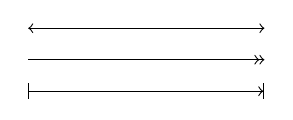
\begin{tikzpicture}[yscale=0.8]
  \draw[<->] (0,-0)--++(3,0);
  \draw[->>] (0,-0.5)--++(3,0);
  \draw[|->|] (0,-1.0)--++(3,0);
\end{tikzpicture}
\end{VerbatimOut}
\ShowExample
%
The \verb|arrows.meta| extension library contains many more tip styles
and options to customize their size; see \cite[Section~16]{tikz}.
%
\begin{VerbatimOut}{\jobname.tmp}
% \usetikzlibrary{arrows.meta}
\begin{tikzpicture}[yscale=0.8]
  \draw[Circle-{Circle[open]}] (0,-0)--++(3,0);
  \draw[-{Stealth[length=5mm,width=2mm,red]}] (4,0)--++(3,0);
  \draw[{->[harpoon]}] (8,0)--++(3,0);
\end{tikzpicture}
\end{VerbatimOut}
\ShowExampleBelow

One more option: the \verb|rounded corners| option does what is says.
It takes as its argument a radius of the corner.
It is one of the few options that can be changed in the middle of a path
(none of the above can, unfortunately).
%
\begin{VerbatimOut}{\jobname.tmp}
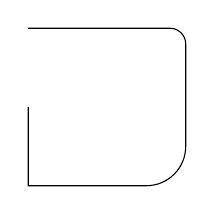
\begin{tikzpicture}
  \draw[rounded corners=2mm] (0,0) -- (2,0)
    [rounded corners=5mm] -- (2,-2)
    [sharp corners] -- (0,-2) -- (0,-1);
\end{tikzpicture}
\end{VerbatimOut}
\ShowExample



%
%
%
\section{Special paths}

In addition to the \verb|--| style path joining two points,
there are the \verb$|-$ and \verb$-|$ styles.
These split the line into vertical and horizontal segments,
the order of which you can probably guess.
%
\begin{VerbatimOut}{\jobname.tmp}
\begin{tikzpicture}
  \draw (0,0) -| (2,1);
\end{tikzpicture}
\end{VerbatimOut}
\ShowExample

To draw rectangles, there is the \verb|rectangle| shorthand
that is put between coordinates of the two opposite corners.
Similarly, there is the \verb|circle| command that is put after the centre coordinate
and takes the radius as an optional parameter.
It is possible to specify \verb|x radius| and \verb|y radius| separately to get an ellipse
(which can be further rotated with the \verb|rotate| parameter).
%
\begin{VerbatimOut}{\jobname.tmp}
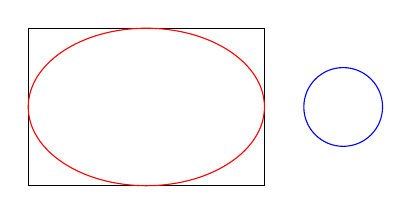
\begin{tikzpicture}
  \draw (0,0) rectangle (3,2);
  \draw[red] (3/2,1) circle
    [x radius=3/2, y radius=1];
  \draw[blue] (4,1) circle [radius=0.5];
\end{tikzpicture}
\end{VerbatimOut}
\ShowExample

There are also commands for drawing arcs, parabolas, and even Bézier curves;
see \cite[Section~14]{tikz}.

There is a helper command for drawing coordinate grids.
TikZ provides a shorthand style \verb|help lines|
that can be customized as in \Cref{sec:tikz styles}.
Here we overlay two grids with different step sizes (default is one unit).
%
\begin{VerbatimOut}{\jobname.tmp}
\centering
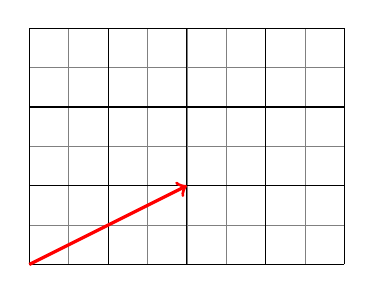
\begin{tikzpicture}
  \draw[help lines, xstep=0.5, ystep=0.5] (0,0) grid (4,3);
  \draw (0,0) grid (4,3);
  \draw[red,very thick,->] (0,0) -- (2,1);
\end{tikzpicture}
\end{VerbatimOut}
\ShowExampleBelow[2]

Now that we know how to draw a coordinate grid,
it is very natural to draw some functions on it!
TikZ includes a reasonably complex calculation engine,
which makes it possible to draw some complicated functions.
%
\begin{VerbatimOut}{\jobname.tmp}
\centering
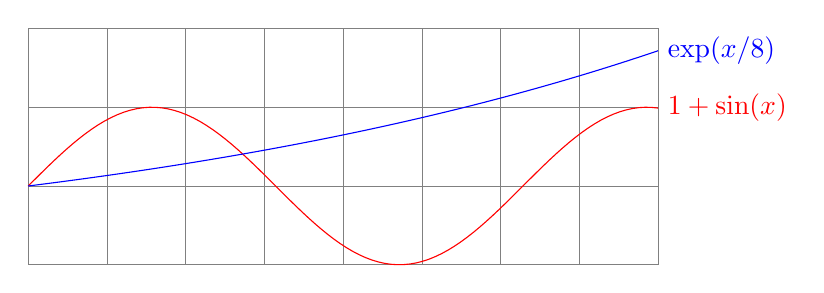
\begin{tikzpicture}
  \draw[help lines] (0,0) grid (8,3);
  \draw[red, domain=0:8, samples=100] plot (\x, {1+sin(\x r)})
    node[right] {$1+\sin(x)$};
  \draw[blue, domain=0:8, samples=100] plot (\x, {exp(\x/8)})
    node[right] {$\exp(x/8)$};
\end{tikzpicture}
\end{VerbatimOut}
\ShowExampleBelow[2]
Some notes on the usage:
\begin{itemize}
\item The domain is specified using the syntax \verb|lower:upper|.
\item The number of samples is optional to specify, but the default value is quite small.
\item The variable $x$ is written with a backslash \verb|\x|,
    but the mathematical commands are spelled without a backslash.
\item Mathematical expressions should be wrapped inside \verb|{}|.
\item Trigonometric functions assume degrees by default;
    the suffix \verb|r| after \verb|\x| converts the variable into radians.
\end{itemize}

Note that the plot is still defined as a pair of $(x,y)$ coordinates.
This makes it possible to draw parametric plots.
The name of the variable can be customized.
%
\begin{VerbatimOut}{\jobname.tmp}
\centering
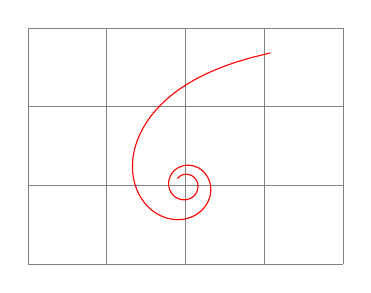
\begin{tikzpicture}
  \draw[help lines] (-2,-1) grid (2,2);
  \draw[red, domain=1:15, samples=150, variable=\t]
    plot ({2*cos(\t r) / \t}, {2*sin(\t r) / \t});
\end{tikzpicture}
\end{VerbatimOut}
\ShowExampleBelow[2]

It is also possible to plot individual points or bar graphs,
or to even load a dataset from an external file.
See \cite[Section~22]{tikz} for more,
but also note the warnings below.

\begin{warning}
``Division by zero'' and ``number too big`` errors
can sometimes lead to confusing (and repeated!) error messages.
\end{warning}

\begin{practices}
TikZ is excellent for producing small and simple function plots
in a style consistent with the rest of the document.
However, compilation times can get quite long for even slightly complicated functions.

I would therefore not recommend using TikZ for complex graphics.
If you still need it, consider disabling the plots in \verb|draft| mode
(by some conditional evaluation; see \Cref{sec:if}).
\end{practices}



%
%
\section{Transformations}

\todo{useasboundingbox}


%
%
\section{Loops}


%
%
\section{Setting styles}\label{sec:tikz styles}


%
%
\section{Some extensions}

\todo{Think about what to cover here: angles, decorations, graphs, trees, spy?}

% !TeX root = 2nd-course-in-latex.tex
\chapter{Presentations with Beamer}

If you ask me, Beamer is an odd tool.
Presentations are inherently visual,
so a programming tool like \LaTeX{} seems ill-suited for the job.
On the other hand, most graphical programs cannot match the quality of \LaTeX{} mathematics,
and technical talks often have modest visual needs.

Beamer does strike a nice balance between the two,
if only your talk is not too ambitious with the visuals.
At the same time I find its complexity to be similar to TikZ
-- a lot of things are possible, but not all of them are advisable.

\begin{practices}
Even though this course is not about presentation skills,
I want to use this opportunity for an important reminder:
Beamer makes it very easy to throw too much mathematics at your audience.

Leave whitespace on your slides, and focus on pictures to support your point.
If you want to dive deep into a mathematical topic,
there is an even superior tool: blackboard.
\end{practices}


%
%
\section{Basic structure}

Beamer is implemented as the \textbf{beamer} document class.
A minimal Beamer file is thus:
%
\begin{ExampleCode}
\documentclass{beamer}

\begin{document}

\begin{frame}
\end{frame}

\end{document}
\end{ExampleCode}
%
Beamer automatically loads \pkg[Beamer]{hyperref}.
It also loads \pkg[Beamer]{amsthm} and creates some theorem environments by default.

Since \TeX{} always believes it is typesetting for printing,
Beamer modifies the page size to be suitable.
By default it is $128 \times 96$~mm, which corresponds to 4:3 aspect ratio.

To modify the aspect ratio, you can pass the \verb|aspectratio| class option.
It is a string of two to four digits, and interpreted like:
\verb|aspectratio=32| means 3:2, \verb|169| means 16:9, and \verb|1610| means 16:10.

\begin{practices}
Many computer screens have 16:9 or 16:10 aspect ratio, so 4:3 might seem old-fashioned.
However, 4:3 has the benefit of increased vertical space.
Many projectors can output either aspect ratio comfortably.
If possible, check the venue beforehand.
\end{practices}

The default 11~pt font fits very nicely with the simulated paper size.
You can pass the \verb|10pt| or \verb|12pt| class options to modify the font size a bit.%
\footnote{There are also some more choices,
but they make the text either very large of very unreadable.}

\begin{gotcha}
You should put \verb|\usefonttheme{professionalfonts}| in the preamble
if you use \mbox{LuaTeX} or XeTeX.
It appears that Beamer does not always recognize that Latin Modern is in use with these compilers.
If the font theme is not changed,
Beamer might produce bad kerning for some specific letter combinations.
\end{gotcha}


For basic title design, you can use the usual \cmd{title}, \cmd{author}, and \cmd{date} commands.
There is also an \cmd{institute} command for specifying the author institution,
and a \cmd{titlegraphic} command that can be used for a logo etc.
Thus a basic presentation with just a title page is set with:
%
\begin{ExampleCode}
\title{My fantastic presentation}
\author{Firstname Lastname}
\institute{University of Puuhamaa}
\titlegraphic{\includegraphics[width=3cm]{TheDogs.jpg}}
\date{20 May 2024}

\begin{document}

\maketitle

\end{document}
\end{ExampleCode}
%
\EmbedPdfPage{examples/basic-beamer.pdf}{1}
%
(The \cmd{maketitle} command can be inside or outside a \verb|frame| environment.
The command is synonymous with \cmd{titlepage}.)

New slides are created with the \env{frame} environments.
Each slide acts like a page, so the basic typesetting commands are available.
The title for the frame can be set with \cmd{frametitle};
it is displayed in the frame header.
%
\begin{ExampleCode}
\begin{frame}
\frametitle{Hi there!}

Welcome to my presentation!

We will talk about Pythagoras and his theorem.
\end{frame}
\end{ExampleCode}
%
\EmbedPdfPage{examples/basic-beamer.pdf}{2}

Note that the paragraphs have no visual separation whatsoever.
You can of course set \cmd[Beamer]{parskip} to a better value
(I suggest a larger value than for printed documents, like 1~em),
but Beamer presentations are often composed of \emph{blocks}.
The \env{block} environment has a title and content:
%
\begin{ExampleCode}
\begin{frame}
\frametitle{Hi there!}

Welcome to my presentation!

\begin{block}{Goal}
You will learn about Pythagoras and his theorem.
\end{block}
\end{frame}
\end{ExampleCode}
%
\EmbedPdfPage{examples/basic-beamer.pdf}{3}
%
In this example the block is not very highlighted,
but that can be changed with a suitable colour theme.
We'll get to that in \Cref{sec:beamer styles}.

By default, Beamer creates a few common theorem environments.
More can be created with the usual \pkg[Beamer]{amsthm} commands (see \Cref{sec:amsthm}).
%
\begin{ExampleCode}
\begin{frame}
\frametitle{The theorem}

\begin{theorem}
If $a$ and $b$ are the lengths of catheti of a right-angled triangle,
then the hypothenuse has length $\sqrt{a^2 + b^2}$.
\end{theorem}
\begin{proof}
We'll get to this soon.
\end{proof}

\end{frame}
\end{ExampleCode}
%
\EmbedPdfPage{examples/basic-beamer.pdf}{4}


To highlight text, it is advisable to use the \cmd{alert} command.
By default it makes the text red, but the style can be customized.

The usual list environments can be used.
Beamer loads the \pkg{enumerate} package that enables a shorthand styling syntax
for \env[shorthand styles]{enumerate} environments.

Let us illustrate these elements with a multi-column layout.
Such a layout is created with a \env[Beamer]{columns} environment.
It takes an optional vertical alignment specifier (top by default;
vertical centres with \verb|c| and bottoms by \verb|b|).%
\footnote{If things do not align as you would expect,
you should also try the \texttt{T} option:
it aligns baselines of the first lines instead of tops of lines.}
%
Inside this environment, columns are created with the \env[Beamer]{column} environment,
which takes column width as a required argument.%
\footnote{There is also an equivalently named command
if you prefer to avoid deeply nested environments.}
%
\begin{ExampleCode}
\begin{columns}
\begin{column}{0.5\textwidth}

Properties of \alert{Pythagoras}:
\begin{enumerate}[1.]
    \item From Ancient Greece ...
\end{enumerate}
\end{column}

\begin{column}{0.5\textwidth}
Properties of \alert{the theorem}:
\begin{enumerate}[i)]
    \item Not invented by Pythagoras ...
\end{enumerate}

\end{column}
\end{columns}
\end{ExampleCode}
%
\EmbedPdfPage{examples/basic-beamer.pdf}{5}


\begin{gotcha}
Frames do not really support the \env[Beamer]{verbatim} environment;
the \pkg{listings} package is probably visually nicer anyways.
\end{gotcha}


%
%
\section{Including graphics}

The usual graphics commands of \LaTeX{} and TikZ can be used as usual.
Moreover, the usual \env[Beamer]{figure} and \env[Beamer]{table} environments can be used.
%
\begin{ExampleCode}
\begin{figure}
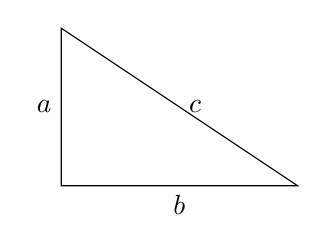
\begin{tikzpicture}
    \draw (0,0) -- (0,2) node[pos=0.5, left] {$a$}
        -- (3,0) node[pos=0.5, right] {$c$}
        -- cycle node[pos=0.5, below] {$b$};
\end{tikzpicture}
\caption{A right triangle.}
\end{figure}

\begin{figure}
    \includegraphics[width=3cm]{TheDogs.jpg}
\caption{Slide hijacked by a dog!}
\end{figure}
\end{ExampleCode}
%
\EmbedPdfPage{examples/basic-beamer.pdf}{6}

\begin{gotcha}
As with article classes, figures are not placed side by side.
The \pkg{subcaption} package is again useful for that;
see \Cref{sec:subfigures}.
Moreover, there is no automatic page breaking:
if you put too much stuff on a slide, they will overflow.
\end{gotcha}


If you need to position graphics absolutely,
you can use the absolute positioning system of TikZ (\Cref{sec:tikz absolute}).
For instance, the following code could be used as the basis of a slide header:
\begin{ExampleCode}
\begin{tikzpicture}[remember picture,overlay]
\node[yshift=0.15\paperheight] at (current page.center){%
\includegraphics[width=\paperwidth]{slideheader.jpg}};
\end{tikzpicture}
\end{ExampleCode}
This assumes the picture to be wide but narrow.
The code needs to be compiled twice before anything is visible.


\begin{warning}
You can find code examples and Beamer documentation about embedding video files inside a presentation.
This is a great way to make a presentation work only on a specific Acrobat Reader version
and only on your current computer.
It is 99~\% guaranteed not to work at a conference venue.

As annoying as it is to switch between programs to show videos,
it is the only reliable option.
\end{warning}

\begin{technote}
As with embedded videos, it is possible to specify slide transition effects,
but they might not work with all PDF viewers.
Because of this, we do not discuss them here.
\end{technote}



%
%
\section{Uncovering things}

The easiest way to uncover things piecewise is the \cmd{pause} command.
As the name suggests, it inserts a slide break at the source location.
%
\begin{ExampleCode}
\begin{frame}
\frametitle{A digression on numbers}

\begin{theorem}
Every natural number has a successor.
\end{theorem}

\pause

\begin{theorem}
There is at least one natural number.
\end{theorem}

\pause

\begin{corollary}
There are infinitely many natural numbers.
\end{corollary}
\end{frame}
\end{ExampleCode}
%
\begin{center}
\fbox{\includegraphics[page=7, width=0.3\textwidth]{examples/basic-beamer.pdf}}~
\fbox{\includegraphics[page=8, width=0.3\textwidth]{examples/basic-beamer.pdf}}~
\fbox{\includegraphics[page=9, width=0.3\textwidth]{examples/basic-beamer.pdf}}
\end{center}

The \cmd{pause} command can be used in many places:
between blocks and paragraphs and inside lists.

\begin{gotcha}
The \cmd{pause} command does not work inside \pkg[with Beamer]{amsmath} environments.
\future{Workarounds?}
\end{gotcha}

To get more control, it is possible to use the \cmd{uncover} command
and \emph{overlay specifications}.\index{overlay specification}
Here are some example overlay specifications:
\begin{description}
\item[\texttt{<2>}] Only shown on slide~2.
\item[\texttt{<2->}] Shown on slide~2 and all following slides.
\item[\texttt{<2-3,5>}] Shown on slides~2--3 and~5.
\end{description}
%
The block environments support overlay specifications,
so the previous example could be rewritten as:
%
\begin{ExampleCode}
\begin{frame}
\frametitle{A digression on numbers, version 2}

\begin{theorem}<1->
Every natural number has a successor.
\end{theorem}

\begin{theorem}<2->
There is at least one natural number.
\end{theorem}

\begin{corollary}<3->
There are infinitely many natural numbers.
\end{corollary}
\end{frame}
\end{ExampleCode}
%
There is also a shorthand syntax \verb|<+->| that is functionally similar to \cmd{pause}:
it increments the previous overlay specification by one.%
\footnote{To be precise, the magic command is \texttt{+}:
it is replaced by the previous slide number, and the slide number is then incremented.}
In the previous example, all overlay specifications could be replaced by \verb|<+->|.
This is particularly useful for lists:
%
\begin{ExampleCode}
\begin{itemize}
    \item<+-> This is shown starting from the first slide.
    \item<+-> This is shown starting from the second slide.
    \item<+-> This is shown starting from the third slide.
\end{itemize}
\end{ExampleCode}
%
Beamer introduces an optional argument to produce such lists with even less repetition:
%
\begin{ExampleCode}
\begin{itemize}[<+->]
    \item This is shown starting from the first slide.
    \item This is shown starting from the second slide.
    \item This is shown starting from the third slide.
\end{itemize}
\end{ExampleCode}

Outside an environment or list, the \cmd{uncover} command works the same:
%
\begin{ExampleCode}
\begin{frame}
\frametitle{On the infinitude of numbers}

\begin{corollary}
There are infinitely many natural numbers.
\end{corollary}
\begin{proof}
\uncover<2->{Suppose that $n$ is the largest natural number.}
\uncover<3->{But then its successor $n+1$ is an even larger natural number.}
\end{proof}

\end{frame}
\end{ExampleCode}
%
\begin{center}
\fbox{\includegraphics[page=10, width=0.3\textwidth]{examples/basic-beamer.pdf}}~
\fbox{\includegraphics[page=11, width=0.3\textwidth]{examples/basic-beamer.pdf}}~
\fbox{\includegraphics[page=12, width=0.3\textwidth]{examples/basic-beamer.pdf}}
\end{center}

Overlay specifications can also be applied to text styling commands like \cmd{alert}.
In this case, the text styling is only applied on the specified frames.
%
\begin{ExampleCode}
\begin{frame}

\textbf<1>{Bold on the first slide only.}\\
\alert<2>{Alerted on the second slide only.}

\end{frame}
\end{ExampleCode}
%
\begin{center}
\fbox{\includegraphics[page=13, width=0.45\textwidth]{examples/basic-beamer.pdf}}~
\fbox{\includegraphics[page=14, width=0.45\textwidth]{examples/basic-beamer.pdf}}
\end{center}

Lists have a special shorthand syntax for setting an element in alerted style.
An overlay specification like \verb|<alert@2>| will make the item alerted on the second slide only.
This can be combined with the \verb|+| syntax to simplify matters:
%
\begin{ExampleCode}
\begin{itemize} % Or put [<alert@+>] here
    \item<alert@+> This is highlighted on the first slide.
    \item<alert@+> This is highlighted on the second slide.
    \item<alert@+> This is highlighted on the third slide.
\end{itemize}
\end{ExampleCode}
%
If necessary, you can combine uncover and alert specifications with syntax like \verb+<1- | alert@2>+,
or the monstrous \verb&<+-|alert@+>& (which alerts on the same slide as where the item appears).

\begin{practices}
The Beamer manual advises against gradually revealing lists,
so making them all visible from the start,
but alerting each item in turn might be a better option.
\end{practices}


There is also an \cmd{only} command.
Its difference to the \cmd{uncover} command is that no space is reserved.
Since it may cause the positioning of the adjacent text change
between slides, it should only be used when necessary.
(This example also has some extra syntax described below.)
%
\begin{ExampleCode}
\begin{frame}<1-2>[label=surprise-dogs]

There is nothing to see here.\\
\only<2>{\includegraphics[width=6cm]{../pictures/TheDogs.jpg}\\}
Absolutely nothing at all.\\
\only<3>{\Large What was that?!}

\end{frame}
\end{ExampleCode}
%
\begin{center}
\fbox{\includegraphics[page=15, width=0.45\textwidth]{examples/basic-beamer.pdf}}~
\fbox{\includegraphics[page=16, width=0.45\textwidth]{examples/basic-beamer.pdf}}
\end{center}

It is possible to repeat a frame without duplicating the code.
In the previous example, we set a label for the frame.
The \cmd{againframe} command can be used to repeat a frame,
even if there were other frames in between.
This mechanism also works together with overlay specifications:
the above example only shows slides 1--2, and the next code shows the final slide:
%
\begin{ExampleCode}
\againframe<3>{surprise-dogs}
\end{ExampleCode}
%
\begin{center}
\fbox{\includegraphics[page=17, width=0.45\textwidth]{examples/basic-beamer.pdf}}
\end{center}


\begin{remark}
You can also uncover parts of a TiKZ picture gradually.
By default TikZ reserves space only for the visible elements;
to avoid elements moving around you can use the \cmd{useasboundingbox} command
we met on page~\pageref{ex:tikz useasboundingbox}.
\end{remark}


\future{reserving space for other elements}

%
%
%
\section{Sections and parts}

The \cmd[Beamer]{section} command can be used to organize your presentation into sections.
In some themes (see \Cref{sec:beamer styles}),
the current section -- and even progress within the section -- is displayed in the header.
As usual, a shorter section name can be passed in an optional argument.

The \cmd{sectionpage} command can be used to set a ``title page'' for the section.
(The default theme used in this example does not set it very beautifully.)
%
\begin{ExampleCode}
\section{Details of the proof}

\sectionpage
\end{ExampleCode}
%
\begin{center}
\fbox{\includegraphics[page=18, width=0.45\textwidth]{examples/basic-beamer.pdf}}
\end{center}

However, it might be more useful to create a frame that shows
the new section highlighted in the table of contents.
This can be achieved with
%
\begin{ExampleCode}
\begin{frame}
    \tableofcontents[currentsection]
\end{frame}
\end{ExampleCode}
%
Without the optional argument, an ordinary table of contents is printed.

It is possible to put ``backup'' slides in an appendix.
Any sections and frames following \cmd[Beamer]{appendix}
will not be shown in navigation bars in the header.

There are also similar subsection-level commands,
if you really need that level of granularity.
In the other end of the granularity spectrum,
the \cmd[Beamer]{part} command can also be used.
Each part is essentially its own isolated presentation
-- the table of contents only shows the current part, and so on.

You can create a bibliography with the manual method described in \Cref{sec:bibliography manual}.
The reason \emph{not} to use BibTeX is that the bibliography
might need to be broken across several frames.
(You can use the \verb|.bbl| file generated by BibTeX as a starting point, of course.)

\begin{practices}
Please think of your audience.
Throwing seventeen references at them in the last 20~seconds of your talk is beyond useless.
Consider using e.g.\ footnotes at the point of citation instead.
\end{practices}




%
%
%
\section{Styling it}\label{sec:beamer styles}

Like the rest of \LaTeX, Beamer attempts to separate content and presentation.
It does so via an extensive styling system.
The appearance of presentation is controlled with commands in the preamble.

First off, controlling the navigation symbols.
There are several styles for them, but I believe you only need one
-- the one where they are not shown:%
\footnote{Have you ever seen anyone use them?}
\begin{ExampleCode}
\beamertemplatenavigationsymbolsempty
\end{ExampleCode}

\begin{remark}
As mentioned above, if you use LuaLaTeX or XeLaTeX,
you should usually also specify
\begin{ExampleCode}
\usefonttheme{professionalfonts}
\end{ExampleCode}
to avoid small kerning issues with some characters.
\end{remark}


Some people prefer to show ``covered'' text in slightly transparent style,
so that the audience sees that it is there.
This can be controlled with the \cmd{setbeamercovered} command.
It takes one argument, and the common values for it are:
\begin{description}
\item[\texttt{invisible}] The default: covered text is invisible.
\item[\texttt{transparent}] Covered text is partially visible.
    This is in fact equivalent to \verb|transparent=15|, where the percentage can be tweaked.
\item[\texttt{dynamic}] The transparency effect depends on the number of slides until the piece is uncovered.
    Use with extreme caution, might be distracting.
\end{description}



%
%
\subsection{Themes}

Beamer comes with a complex theming system for changing the appearance of things.
Essentially, you should only need to modify the preamble to change how things look.

The overall appearance is determined by the \emph{presentation theme}.
It is chosen with \cmd{usetheme} in the preamble.
The presentation theme, in turn, consists of four parts, any of which can be changed independently:
\begin{description}
\item[Inner theme] The appearance of frame contents (blocks, lists, etc.)
    Changed with \cmd{useinnertheme}.
\item[Outer theme] The appearance of frame border (footer, navigation bar etc.)
    Changed with \cmd{useoutertheme}.
\item[Color theme] The colours used for elements.
    Individual colours can be further customized.
    Changed with \cmd{usecolortheme}.
\item[Font theme] The fonts to be used for elements.
    Also these can be customized individually.
    Changed with \cmd{usefonttheme}.
\end{description}
%
It is thus possible to start from a presentation theme,
and then change parts of the style to suit your artistic tastes.

The built-in presentation themes are showcased in \cite[Chapter~15]{beamer},
inner and outer themes in \cite[Chapter~16]{beamer},
and color and font themes in the following chapters.

In this example, we use the \verb|Madrid| presentation theme without any further customization:%
\footnote{Except for using \texttt{professionalfonts}, since the file was compiled with XeLaTeX.}
%
\begin{ExampleCode}
\title{My fantastic presentation}
\author[F.~Lastname]{Firstname Lastname}
\institute[U.~Puuhamaa]{University of Puuhamaa}
\date{20 May 2024}

\beamertemplatenavigationsymbolsempty
\usefonttheme{professionalfonts}
\usetheme{Madrid}
\end{ExampleCode}
%
\begin{center}
\fbox{\includegraphics[page=1, width=0.45\textwidth]{examples/beamer-theme.pdf}}~
\fbox{\includegraphics[page=2, width=0.45\textwidth]{examples/beamer-theme.pdf}}
\end{center}

Then, let us modify the look a bit.
We take the \verb|miniframes| outer theme into use;
it displays the sections and progress within section in the header.
We also use its optional argument to simplify the footer.
We then change to the \verb|crane| colour theme in order to induce a headache in our audience,
and use the default serif font:
%
\begin{ExampleCode}
\beamertemplatenavigationsymbolsempty
\usefonttheme{professionalfonts}
\usetheme{Madrid}
\useoutertheme[footline=authortitle]{miniframes}
\usecolortheme{crane}
\usefonttheme{serif}
\end{ExampleCode}
%
\begin{center}
\fbox{\includegraphics[page=1, width=0.45\textwidth]{examples/beamer-theme2.pdf}}~
\fbox{\includegraphics[page=2, width=0.45\textwidth]{examples/beamer-theme2.pdf}}
\end{center}



%
%
\subsection{Colours}

\begin{practices}
It is \emph{extra important} to take care of colour contrast in presentations.
Projectors have a far smaller colour range than computer displays,
especially if the room is bright.
What might appear like two distinct colours on your laptop
might be indistinguishable when projected.
\end{practices}

If the colour scheme provided by \cmd{usecolortheme} is still not what you want,
it is possible to tweak the individual colours.
This is done with \cmd{setbeamercolor}.

Beamer uses named colours for everything.
For example, the \verb|block body| colour is used inside all \env{block} environments.
Each colour also has two components: foreground (\verb|fg|) and background (\verb|bg|).
These can be set to any values supported by \pkg{xcolor}.

For example, here we change the foreground colour of block titles,
and both the foreground and background colours of block bodies:%
\begin{ExampleCode}
\setbeamercolor{block title}{fg=red}
\setbeamercolor{block body}{fg=white, bg=blue}
\end{ExampleCode}
%
\begin{center}
\fbox{\includegraphics[page=3, width=0.6\textwidth]{examples/beamer-theme2.pdf}}
\end{center}

Some of these colours are also inherited from ``parent colours''.
Maybe the most interesting of these is \verb|structure|,
which applies to all frame and block headings, unless overridden by a child style.
The colour of the ``background canvas'' is determined by the \verb|bg| colour of \verb|normal text|.

You can find the full list of predefined colours in the Beamer documentation for each element type.
The source code of each Beamer colour theme is also very readable,
and can be used as a reference.%
\footnote{Where your particular \LaTeX{} installation puts package sources might be complicated.
For Beamer, the source is also available on Github:
\url{github.com/josephwright/beamer}.}



\subsection{Fonts}

\begin{practices}
Beamer uses a sans-serif font by default.
This is a good choice since sans-serif fonts are usually more readable in low resolution.
However, a serif font can be used to give a nice classic look.

Using \emph{italic} for emphasis might be too subtle;
prefer alerted and boldface text in presentations.
\end{practices}

As with colours, Beamer comes with a few built-in font themes
accessible with \cmd{usefonttheme}.
In addition to the \verb|professionalfonts| mentioned above
(which just disables some internal features, and can be used together with another font theme),
there is the sans-serif \verb|default|, its counterpart \verb|serif|,
and a few others that modify headings only \cite[Section~18.1]{beamer}.

The font size is controlled with the package options.
Moreover, since Beamer uses the default serif and sans-serif fonts,
you can replace the fonts with the methods described in \Cref{sec:typefaces}.

If you really need to customize the font used for a particular element,
there is a system similar to the one used for colours.
The \cmd{setbeamerfont} command takes the element name and a list of attributes to override.
The attributes are \verb|size|, \verb|shape|, \verb|series|, and \verb|family|,
and their possible values are the declarations listed in \Cref{sec:font attributes}.

In this (now awfully ugly) example,
we modify the frame title to be in bold, sans-serif font:
\begin{ExampleCode}
\setbeamerfont{frametitle}{series=\bfseries, family=\sffamily}
\end{ExampleCode}
%
\begin{center}
\fbox{\includegraphics[page=4, width=0.6\textwidth]{examples/beamer-theme2.pdf}}
\end{center}



%
%
\subsection{Templates}

Finally, the appearance of repeated elements like titles can be controlled by \emph{templates}.
Since this goes deeper into the internals of Beamer,
we only refer to the documentation \cite[Section~16.3]{beamer}.


%
%
\section{Handouts}

To produce handouts, pass the \verb|handout| optional argument to the document class.
In this mode, the overlays are ``flattened'' so that everything is visible at once.

If you still need to split a frame into multiple parts in the handout,
you can modify the overlay specification to also apply to handouts.\index{overlay specification!handout}
The following code shows its contents on the third slide in presentation mode,
and on the second slide in handout mode:
\begin{ExampleCode}
\only<3|handout:2>{...}
\end{ExampleCode}

To suppress the inclusion of a frame,
you can put \verb|<handout:0>| immediately after \verb|\begin{frame}|.
This overlay specification means that only the 0th slide of the frame will be printed in the handout
-- which does nothing, since the slide numbers start at 1.


\chapter{Posters with tikzposter}

There are several methods to creating posters with \LaTeX{}.
To mention just three of the many packages: \pkg{tikzposter}, \pkg{beamerposter}, and \pkg{tcolorbox}.
All of them suffer from the fact that posters are very visual,
but \TeX{} can really only do boxes.

Here we discuss \pkg{tikzposter} since it is reasonably simple.
However, the package has not been actively maintained since~2014,
and it appears to have some bugs.
The other packages use fairly similar principles.


%
%
\section{Basic layout}

The package is loaded with
%
\begin{ExampleCode}
\documentclass{tikzposter}
\end{ExampleCode}
%
By default, the options \verb|a0paper|, \verb|25pt|, and \verb|portrait| are used.
Paper sizes A1 and A2 are also available, and the \verb|landscape| option produces a landscape page.
The range of font sizes is limited to 12, 14, 17, 20, and 25~points.
Of these, only the last one is suitable for A0~size.

\begin{practices}
As with presentations, you should not have too much text.
Use whitespace and structure to guide the reader.
\end{practices}

For one reason or other, the package adds a watermark to the lower-right corner.
It can be turned off with the monstrously long command
%
\begin{ExampleCode}
\tikzposterlatexaffectionproofoff
\end{ExampleCode}
%
There are also some package options to control margins and default block spacing;
see the documentation for details.

The title is set with \cmd[tikzposter]{maketitle} as usual;
you can set \cmd{title}, \cmd{author}, and \cmd{institute} in the preamble.
You can also put graphical (or rather, any) commands inside \cmd{titlegraphic}.
By default these elements are set on top of each other.
The customization is briefly discussed in \Cref{sec:poster style}.
The \cmd[tikzposter]{maketitle} command also accepts some optional arguments like
%
\begin{ExampleCode}
\maketitle[width=40cm]
\end{ExampleCode}



As with Beamer, the basic layout consists of blocks.
The \cmd[tikzposter]{block} command takes optional customization arguments,
a title, and the contents:
%
\begin{ExampleCode}
\block[]{Block title goes here}
{
Contents of the block
}
\end{ExampleCode}
%
The block will fill the available horizontal space,
and the vertical size depends on the contents.
Contents can be any material (except floats).
If the title is empty, the ``block header'' disappears.

To set several blocks side by side, it is possible to use columns
specified inside a \env{tikzposter}{columns} environment.
A new column is started with the \cmd[tikzposter]{column} command.
As its argument it takes the fraction of text area width.%
\footnote{You need to ensure that they sum to at most $1$.
The documentation also talks about absolute widths, but they do not seem to actually work.}
Any blocks specified after this command will be placed vertically in the column.
For example, here we set two columns of equal size,
and place two blocks in the left column:
%
\begin{ExampleCode}
\begin{columns}

\column{0.5}
\block{Above left}{}
\block{Below left}{}

\column{0.5}
\block{Right}{}

\end{columns}
\end{ExampleCode}

The \env[tikzposter]{subcolumns} and \cmd[tikzposter]{subcolumn}
can be used to further divide a column
(the arguments are fractions of the \emph{outer column} width).

After the \env{columns} environment ends,
all new blocks again fill the whole horizontal space.

You cannot use the usual vertical spacing commands to adjust spacing between blocks.
A workaround is to add an offset both to the block title and contents.
Negative $y$ values point downwards.%
\footnote{It appears that this method might not work with blocks without title;
this seems to be a bug.}
%
\begin{ExampleCode}
\block[titleoffsety=-2cm, bodyoffsety=-2cm]{Title}{Contents}
\end{ExampleCode}

Inside a block, you can use the \cmd[tikzposter]{coloredbox} command to create highlighted regions.
%
\begin{ExampleCode}
\block{Goal}
{
In this poster we discuss Pythagoras' theorem.

\coloredbox{It is maybe the most important theorem in human history!!}

\coloredbox[bgcolor=PeachPuff, fgcolor=red]{\centering I mean it!!!}
}
\end{ExampleCode}
%
It is also possible to add small notes.
They are defined outside blocks, but they attach to the previous block.
By default, they connect to the center of the block,
but the precise point can be adjusted with optional arguments,
as with the distance and angle (here east-southeast) to the anchor point:
%
\begin{ExampleCode}
\note[angle=-20, radius=8cm, connection, targetoffsety=-2cm]
    {This poster will convince you about it!}
\end{ExampleCode}

Let us see how these pieces (and a few more content additions) play together.
The output of the following code is shown in \Cref{fig:poster example}.

\begin{figure}
\centering
\includegraphics[height=0.85\textheight]{examples/tikzposter-content.pdf}
\caption{The example poster (set in A2 size, and scaled here).}\label{fig:poster example}
\end{figure}

\VerbatimInput[fontsize=\footnotesize,frame=lines]{examples/tikzposter-content.tex}




%
%
\section{Styling}\label{sec:poster style}

The styling system of \pkg[styling]{tikzposter} is very similar to that of Beamer.
There are a few built-in styles.%
\footnote{\url{https://bitbucket.org/surmann/tikzposter/downloads/styleguide.pdf}}


\begin{technote}
The source code for the predefined styles is very readable.
If you want to customize styles, I recommend using their code as a starting point.

The installation location of packages depends on your specific \LaTeX{} installation,
but the code can also be browsed online at \url{https://bitbucket.org/surmann/tikzposter/}.
\end{technote}


The overall look is controlled by \cmd[tikzposter]{usetheme},
and then e.g.\ the colour and background styles can be customized.
Individual colours can be changed with \cmd[tikzposter]{colorlet}
(unlike in Beamer, colours are not separated into foreground and background colours).

For example, this code selects the theme in \Cref{fig:poster styled}:
\begin{ExampleCode}
\usetheme{Envelope} % Block and title style set by this
\usecolorstyle{Denmark} % Red-white colour scheme

\usebackgroundstyle{VerticalGradation} % Vertical gradient...
\colorlet{backgroundcolor}{blue!40} % ...with a faint blue colour
\end{ExampleCode}

To modify the layout of the title contents,
it is unfortunately necessary to go to low-level \LaTeX{} code.
The \cmd[tikzposter]{settitle} command can be used to define the layout code for the title contents.
The variables set by the \verb|\maketitle| companion commands can be used as below.
The following code is also used in \Cref{fig:poster styled}:
%
\begin{ExampleCode}
\settitle{
    \makebox[8cm][c]{\@titlegraphic}
    \parbox[b]{20cm}{
        \color{titlefgcolor} {\bfseries \Huge \sc \@title \par}
        \vspace*{1em}
        {\huge \@author{} \Large (\@institute)}
    }
}
\end{ExampleCode}

\begin{figure}
\centering
\includegraphics[height=0.85\textheight]{examples/tikzposter-style.pdf}
\caption{A styled version of the previous example.}\label{fig:poster styled}
\end{figure}



\printindex

\end{document}
